\documentclass[12pt,a4paper]{article}
\usepackage[table]{xcolor}
\usepackage{float}
\usepackage[spanish]{babel}
\usepackage{amsmath}
\usepackage{amssymb}
\usepackage{graphicx}
\usepackage{amsfonts}
\usepackage[utf8]{inputenx}
%\usepackage{algorithm2e}
\usepackage{listings}
\usepackage{pdfpages}
\usepackage{tabularx}
\usepackage{color}
\usepackage{anysize}
\usepackage{fancyhdr}
\usepackage{ulem}
%\usepackage{caption}
\usepackage[font=footnotesize]{caption}
\definecolor{deepblue}{RGB}{0,0,153}
\definecolor{deepred}{RGB}{153,0,0}
\definecolor{deepgreen}{RGB}{51,102,0}
\definecolor{deepyellow}{RGB}{204,204,0}
\marginsize{2cm}{2cm}{1cm}{1.5cm} % depende de anysize
%\renewcommand*{\thefootnote}{\Roman{footnote}}
\lstset{ %
			language=Python,
			basicstyle=\footnotesize,
			numbers=left,
			stepnumber=1,
			numbersep=4pt,
			tabsize=2,
			otherkeywords={self}, 
			keywordstyle=\color{deepred},
			stringstyle=\color{deepgreen},
			commentstyle=\color{deepblue},
}
\usepackage{hyperref}
\hypersetup{
    colorlinks=true,
    citecolor=black,
    filecolor=black,
    linkcolor=black,
    urlcolor=black,
    linktoc=all
}



%\title{Multímetros en Corriente Continua}
\title{TP Final}
\author{
        Grupo 1
}
\date{\today}
\pagestyle{fancy}
\lhead{Facultad de Ingenieria}
\rhead{Laboratorio - 66.02 - Curso 001 - TP Final}


\begin{document}
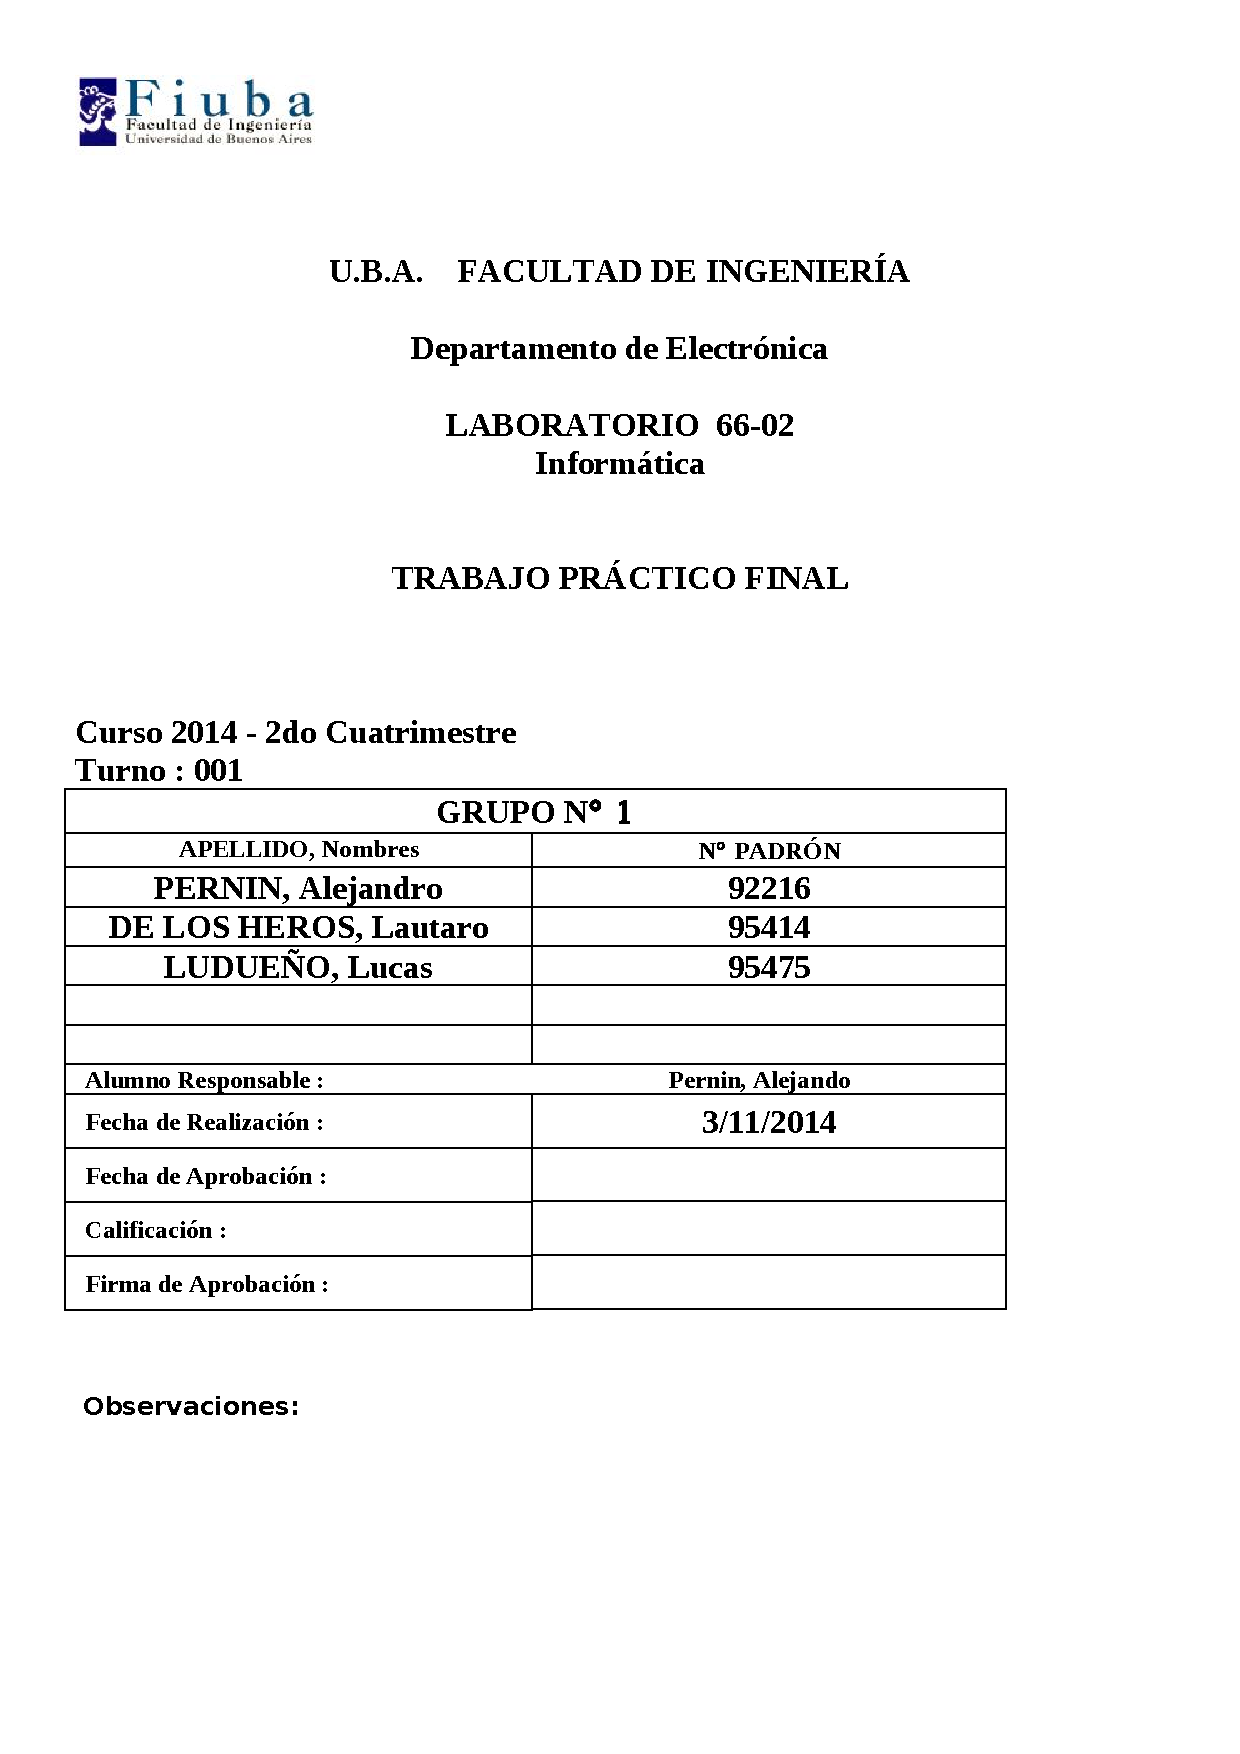
\includepdf{attachments/caratula.pdf}


\newpage\null\thispagestyle{empty}\newpage

\maketitle
\newpage\null\thispagestyle{empty}\newpage

\newpage
\tableofcontents

\newpage\null\thispagestyle{empty}\newpage

\newpage


\newpage 
\section{Introducción}
	El objetivo de este informe es exponer el trabajo práctico final, mostrando los desarrollos, mediciones efectuadas, funcionamiento y decisiones tomadas durante la confección del mismo. Éste fue realizado a lo largo del cuatrimestre en paralelo con las clases prácticas y los otros trabajos prácticos. Todos los archivo aquí utilizados, incluyendo este informe y su fuente estarán disponibles en \url{http://github.com/aleperno/labotpfinal}. Adicionalmente habrán disponibles algunos videos en YouTube con filmaciones de determinadas mediciones, por lo que es recomendable tener este informe en formato digital para fácil acceso a dichos links.

%	\subsection{Opciones Disponibles}
%		Habiendo diversas alternativas de proyectos de TPs para elegir, en un principio no estuvo del todo claro cuál elegir ya que todos tenian sus complicaciones y objetivos. Algunas de las alternativas disponibles eran la confección de una fuente, un sensor, etc.

	\subsection{Opción Elegida}
		Como proyecto base decidimos desarrollar un voltímetro vúmetro disponible en los cursos de CEKIT \footnote{Pdf del proyecto oringal \url{https://github.com/aleperno/labotpfinal/raw/master/cekit.pdf}}. Elegimos este proyecto ya que si bien se trata de un proyecto relativamente sencillo, tiene aplicaciones reales tanto industriales como hogareñas.

		Además aprovechando que uno de los integrantes poseía un Arduino \footnote{\url{http://arduino.cc/}} y una Raspberry \footnote{\url{http://www.raspberrypi.org/}} decidimos como opcional escalar el proyecto utilizando dichos elementos. En el informe se desarrollará el proyecto base y el opcional se detallará en la sección \ref{sec:escalabilidad} de escalabilidad del proyecto.

		El vúmetro consiste en un arreglo de LEDs que se van encendiendo conforme aumenta la tensión mensurada, la relación entre la cantidad de LEDs encendidos y la tensión proviene de las características intrínsecas del circuito cuyo análisis es parte de este informe. En este proyecto no sólo se implementan las nociones aprendidas tanto en las clases teóricas  como en los TPs realizados, sino que además se emplearon nociones de diseño y elaboración de circuitos y software; por lo que es válido decir que este es un proyecto integrador.

	\subsection{Contenido}
		Breve explicación de los capítulos subsiguientes
		\begin{itemize}
			\item \textbf{Circuito Esquemático} Circuito esquemático del proyecto, con su código fuente incluido.
			\item \textbf{Diagrama de Bloques} Abstracción de los elementos más importantes del circuito con una breve explicación de sus funciones.
			\item \textbf{Desarrollo} Se analizará analíticamente el circuito previo a su confección, elaborando hipótesis que luego seran corroboradas o refutadas mediante mediciones mostrando el funcionamiento y comportamiento del proyecto.
			\item \textbf{Escalabilidad} Se plantean las posibilidades de expansión de circuito, desarrollando algunas de ellas al igual que el proyecto realizando hipótesis, análisis y mediciones.
			\item \textbf{Conclusiones} Conclusiones generales del TP, incluyendo lo aprendido y toda información significativa que surgió del desarrollo del proyecto.
			\item \textbf{Referencias} Referencias hacia los datos o elementos utilizados.
			\item \textbf{Anexo} Información adicional y más completa de especificaciones mencionadas en el desarrollo del TP.
		\end{itemize}

	\newpage
	\section{Circuito Esquemático}
		El circuito implementado es el siguiente \footnote{.sch disponible en \url{https://github.com/aleperno/labotpfinal/raw/master/labo.sch}}:

		\begin{figure}[H]
			\centering
			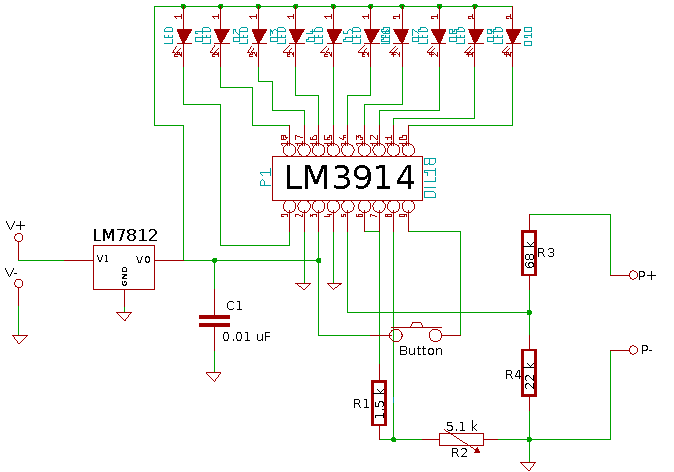
\includegraphics[scale=1.2]{images/sch.pdf}\caption{Esquemático del Circuito}
			\label{fig:circesq}
		\end{figure}

	\section{Diagrama de bloques}

		\begin{figure}[H]
			\centering
			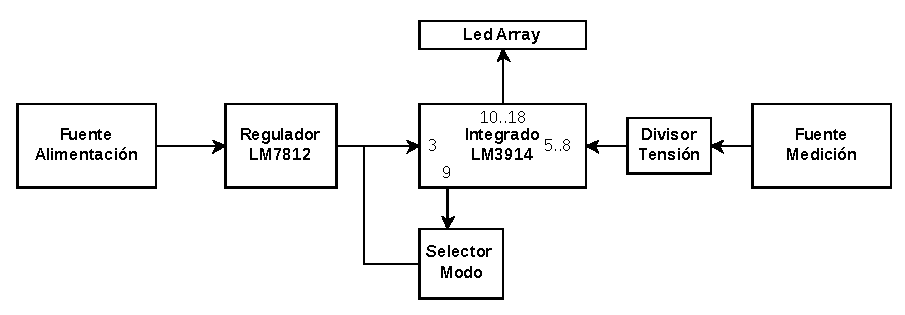
\includegraphics[scale=1.2]{images/bloque.pdf}\caption{Diagrama de Bloques}
			\label{fig:bloque}
		\end{figure}

	\begin{itemize}
		\item \textbf{Fuente de Alimentación:} La fuente que alimenta el circuito, ésta debe ser de al menos 14 V ya que el regulador de tensión es de 12V.
		\item \textbf{Regulador de Tensión LM3914:} El regulador cumple la función de mantener el equipo alimentado con 12 V, evitando daños si la entrada es mayor.
		\item \textbf{Selector Modo:} Nos permite seleccionar ambos modos de funcionamiento del circuito, tanto en "DOT" (se prende un sólo LED), como "BAR" (Se prende consecutivamente el array).
		\item \textbf{Fuente Medición:} Es la fuente de tensión a mensurar.
		\item \textbf{Divisor de Tensión:} Siendo que el integrado posee un límite de 5 V de entrada a medir, se coloca un divisor de tensión para ajustar la tensión a las especificaciones.
		\item \textbf{Array de LEDs:} Es el arreglo de LEDs luminosos en si, en este caso consiste de 10 LEDs.
		\item \textbf{Integrado LM3914: } Es el integrado encargado de la lógica del circuito.

		La fuente de alimentación alimenta el regulador de tensión, obteniéndose en la salida del mismo 12 V estables que alimentan el circuito. Asimismo el divisor de tensión ajusta la tensión aplicada por la fuente a mensurar para que la misma esté dentro de los límites del integrado. El integrado LM3914 es el encargado de la lógica del circuito, al ir incrementando la tensión mensurada, se van incrementando la cantidad de leds (o la posicion del led) encendidos en el array.
	\end{itemize}

	\section{Desarrollo}
		Como primera instancia se debió analizar cuales serían los alcances del proyecto y ajustar las características del circuito al mismo. Lo principal a definir fue el rango de tensiones que mediriámos, decidimos utilizar el mismo rango utilizado como ejemplo en el proyecto orignal, comprendido entre los 0 y 25 V.

		Acorde al datasheet del integrado \footnote{Ver sección \ref{sec:referencias}.} el resistor $R_1$ es el encargado de regular la luminosidad de los LED. Asimismo se establece como corrientes de salida hacia los LED de un mínimo de 7 mA y un típico de 10 mA, para el proyecto establecimos un valor intermedio en $8.3$ mA. Siendo la tensión interna de referencia de $1.25$ V, por la ley de Ohm podemos calcular

		\begin{equation}
			R_1 = \frac{1.25 \: V * 10 \: LED}{8.3 \: mA} \cong 1.5 \: k \Omega
		\end{equation}

		Luego es preciso establecer un fondo de escala, la misma se calcula acorde la siguiente fórmula:

		\begin{equation}\label{eq:vref}
			V_{ref} = 1.25 \: V (1+\frac{R_2}{R_1})
		\end{equation}

		Siendo la máxima señal de entrada permitida de 5 V, para poder mensurar el rango antes mencionado (0 - 25 V) debemos emplear un divisor de tensión, para tal propósito se emplearon los resistores $R_3 = 68 \: k\Omega$ y $R_4 = 22 \: k\Omega$. Acorde a estos valores, aplicando una tensión de 25 V, sobre $R_4$ se obtendrá una caída de tensión equivalente a

		\begin{equation}
			\Delta V_{R_4} = \frac{25 \: V * 22 \: k\Omega}{90 \: k\Omega} \cong 6.1 \: V
		\end{equation}

		Si consideramos la tensión máxima de referencia, según la ecuacion \ref{eq:vref}:

		\begin{equation}
			\displaystyle R_2 = \left.  \left ( \frac{V_{ref}}{1.25 \: V}-1 \right ) * R_1 \right |_{V_{ref} = 5 \: V} = 4.5 \: k\Omega
		\end{equation}

		Siendo este resistor de un valor no comercial y con el fin de a posteriori poder realizar ajustes, empleamos un resistor variable de $10 \: k\Omega$. Teniendo todos los elementos principales ya descriptos, se prosiguió al diseño y confección del circuito.

		%Sin embargo al tener también interactuando un divisor de tensión (y resistores no exactos), empleamos un resistor variable de $10 \: k\Omega$ y aplicando una tensión de 25 V variamos la resistencia, procurando que a los 25 V se encienca el décimo LED. Una vez hecho esto, se midió la resistencia del resistor dando como resultado:

		%\begin{equation}
		%	R_2 = (3.87 \pm 0.05) \: k\Omega
		%\end{equation}

		\subsection{Construcción}

			Como primer instancia luego de adquirir todos los elementos, se armó el circuito en un \textit{protoboard} a fin de corroborar el funcionamiento de todos los componentes individual y conjuntamente.

			\begin{figure}[H]
			\centering
				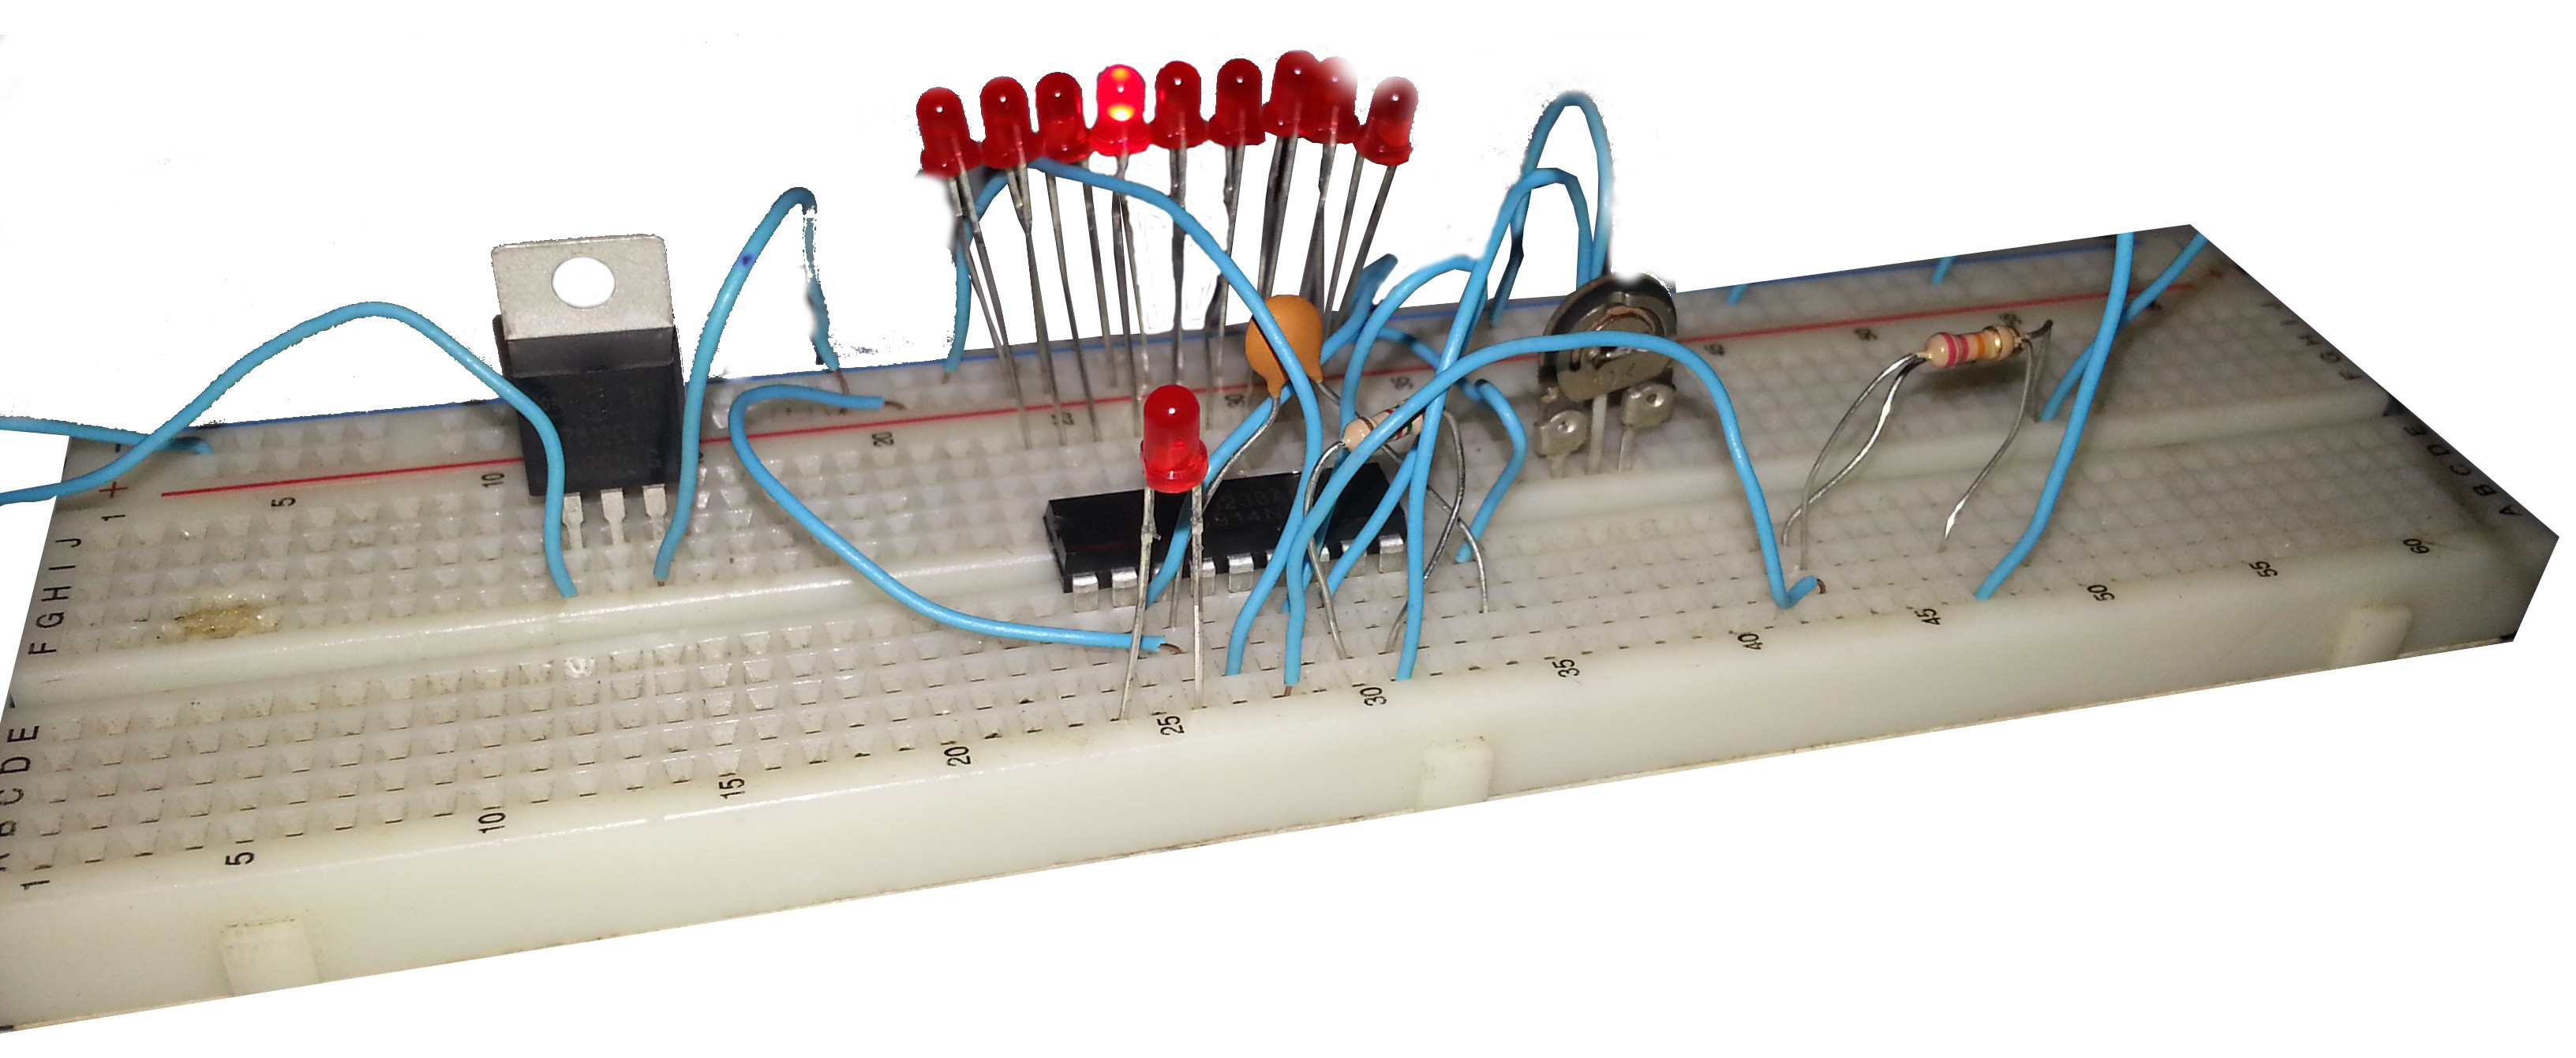
\includegraphics[scale=0.1]{images/proto_dot.jpg}\caption{Prototipo modo DOT}
			\end{figure}

			\begin{figure}[H]
			\centering
				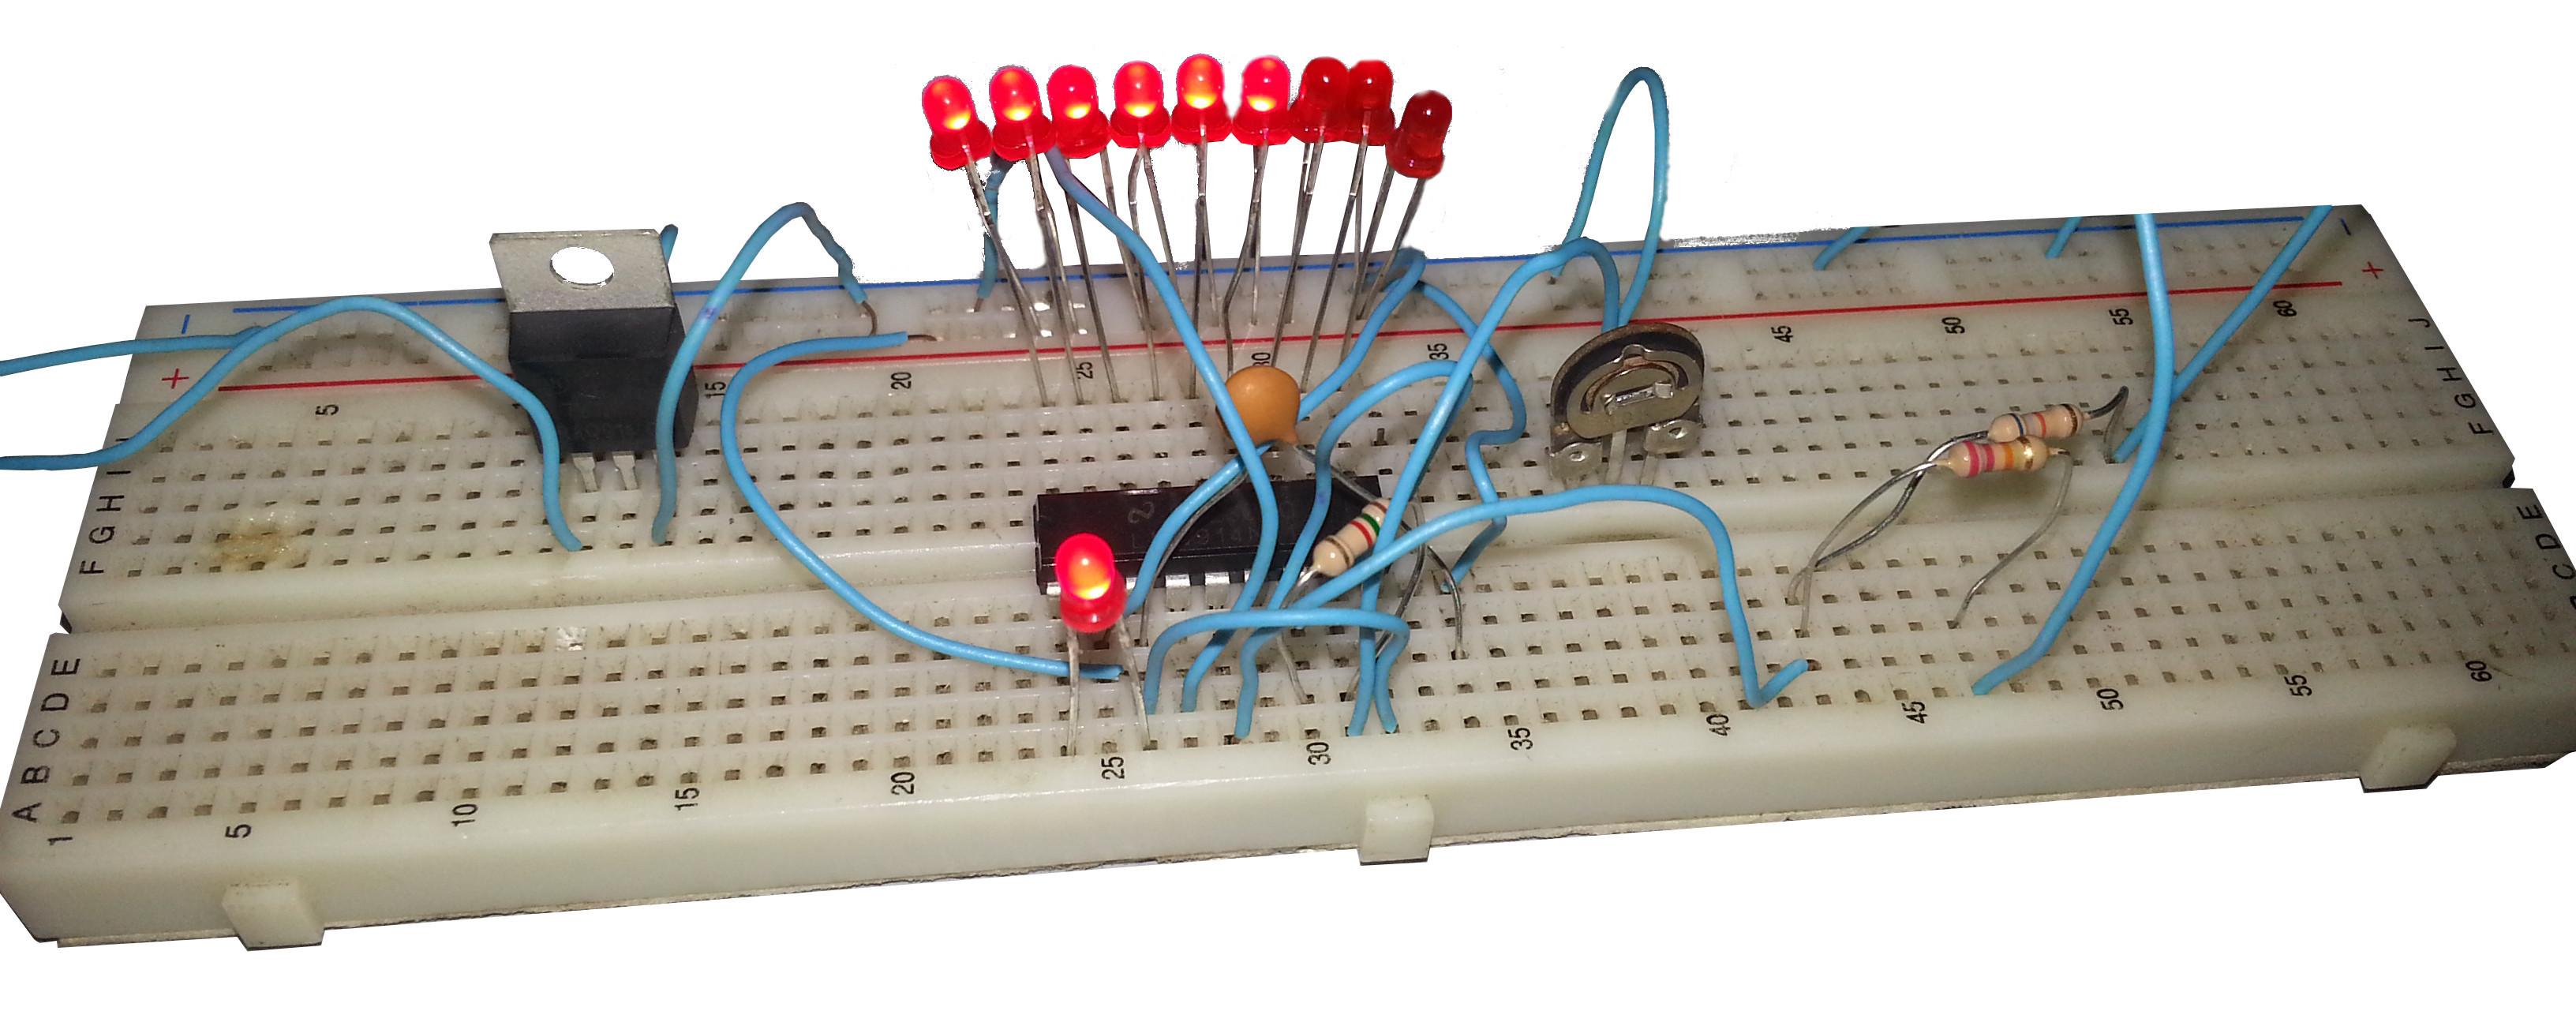
\includegraphics[scale=0.1]{images/proto_bar.jpg}\caption{Prototipo modo BAR}
			\end{figure}

			Luego aprovechando la disponibilidad de un archivo esquemático, utilizando herramientas informáticas se diseñó un circuito virtual que luego sería pasado a una plaqueta de cobre.

			\begin{figure}[H]
			\centering
				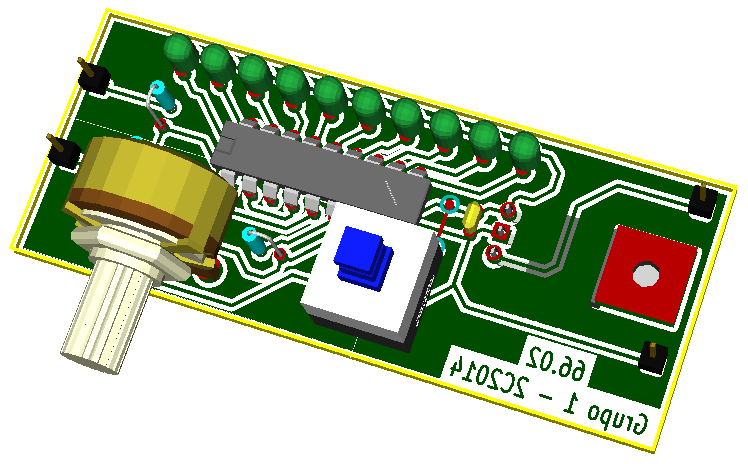
\includegraphics[scale=0.4]{images/virt_sup.png}\caption{Vista Superior Circuito Virtual}
			\end{figure}

			\begin{figure}[H]
			\centering
				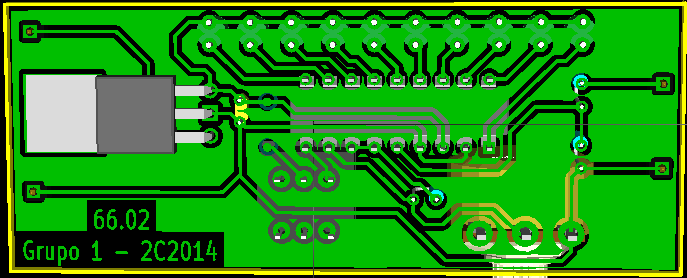
\includegraphics[scale=0.4]{images/virt_inf.png}\caption{Vista Inferior Circuito Virtual}
			\end{figure}

			Una vez conformes con el diseño, se imprimió el mismo en papel de transferencia térmico, para ser pasado a una plancha de cobre virgen y empleando ácido grabar el dibujo en la placa.

			\begin{figure}[H]
			\centering
				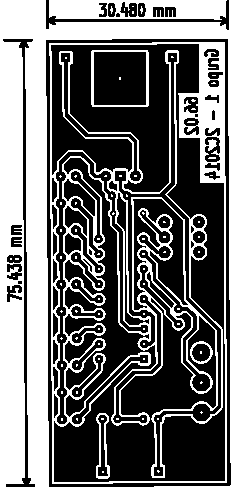
\includegraphics[scale=1,angle=-90]{images/design.pdf}\caption{Diseño Circuito}
			\end{figure}

			\begin{figure}[H]
			\centering
				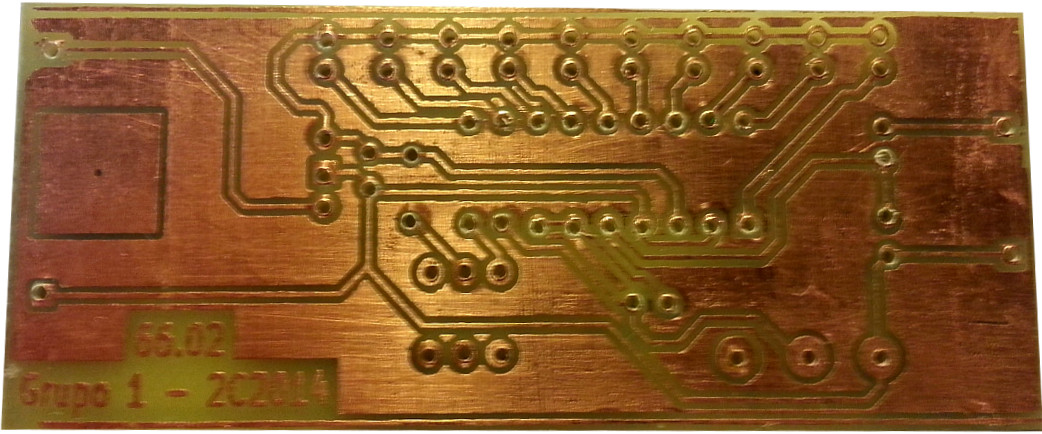
\includegraphics[scale=0.25]{images/placa_grabada.jpg}\caption{Diseño Grabado}
			\end{figure}

			\begin{figure}[H]
			\centering
				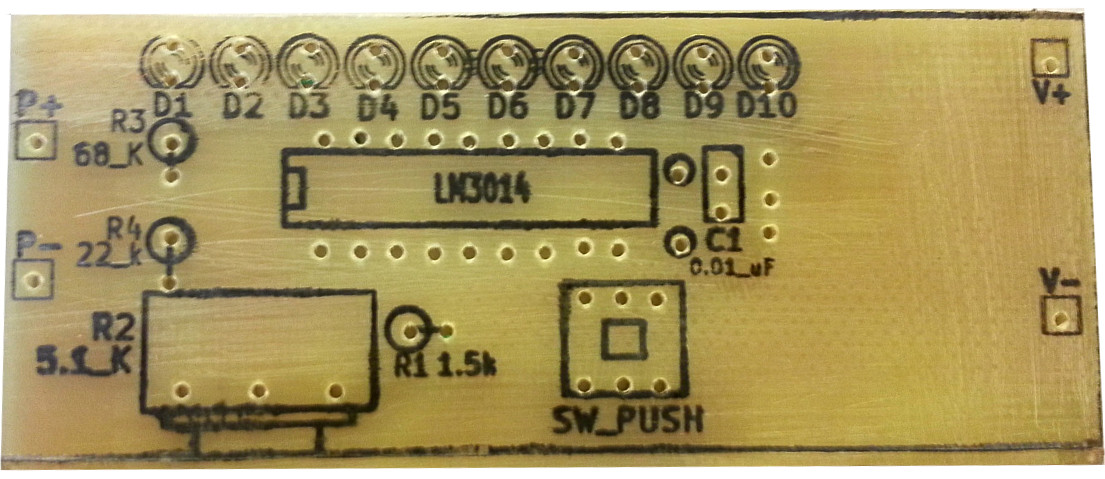
\includegraphics[scale=0.25]{images/ayuda_comps.jpg}\caption{Indicador de Componentes}
			\end{figure}

			Luego de soldar los componentes y realizar algunas reparaciones en las pistas de cobre, el circuito definitivo:

			\begin{figure}[H]
			\centering
				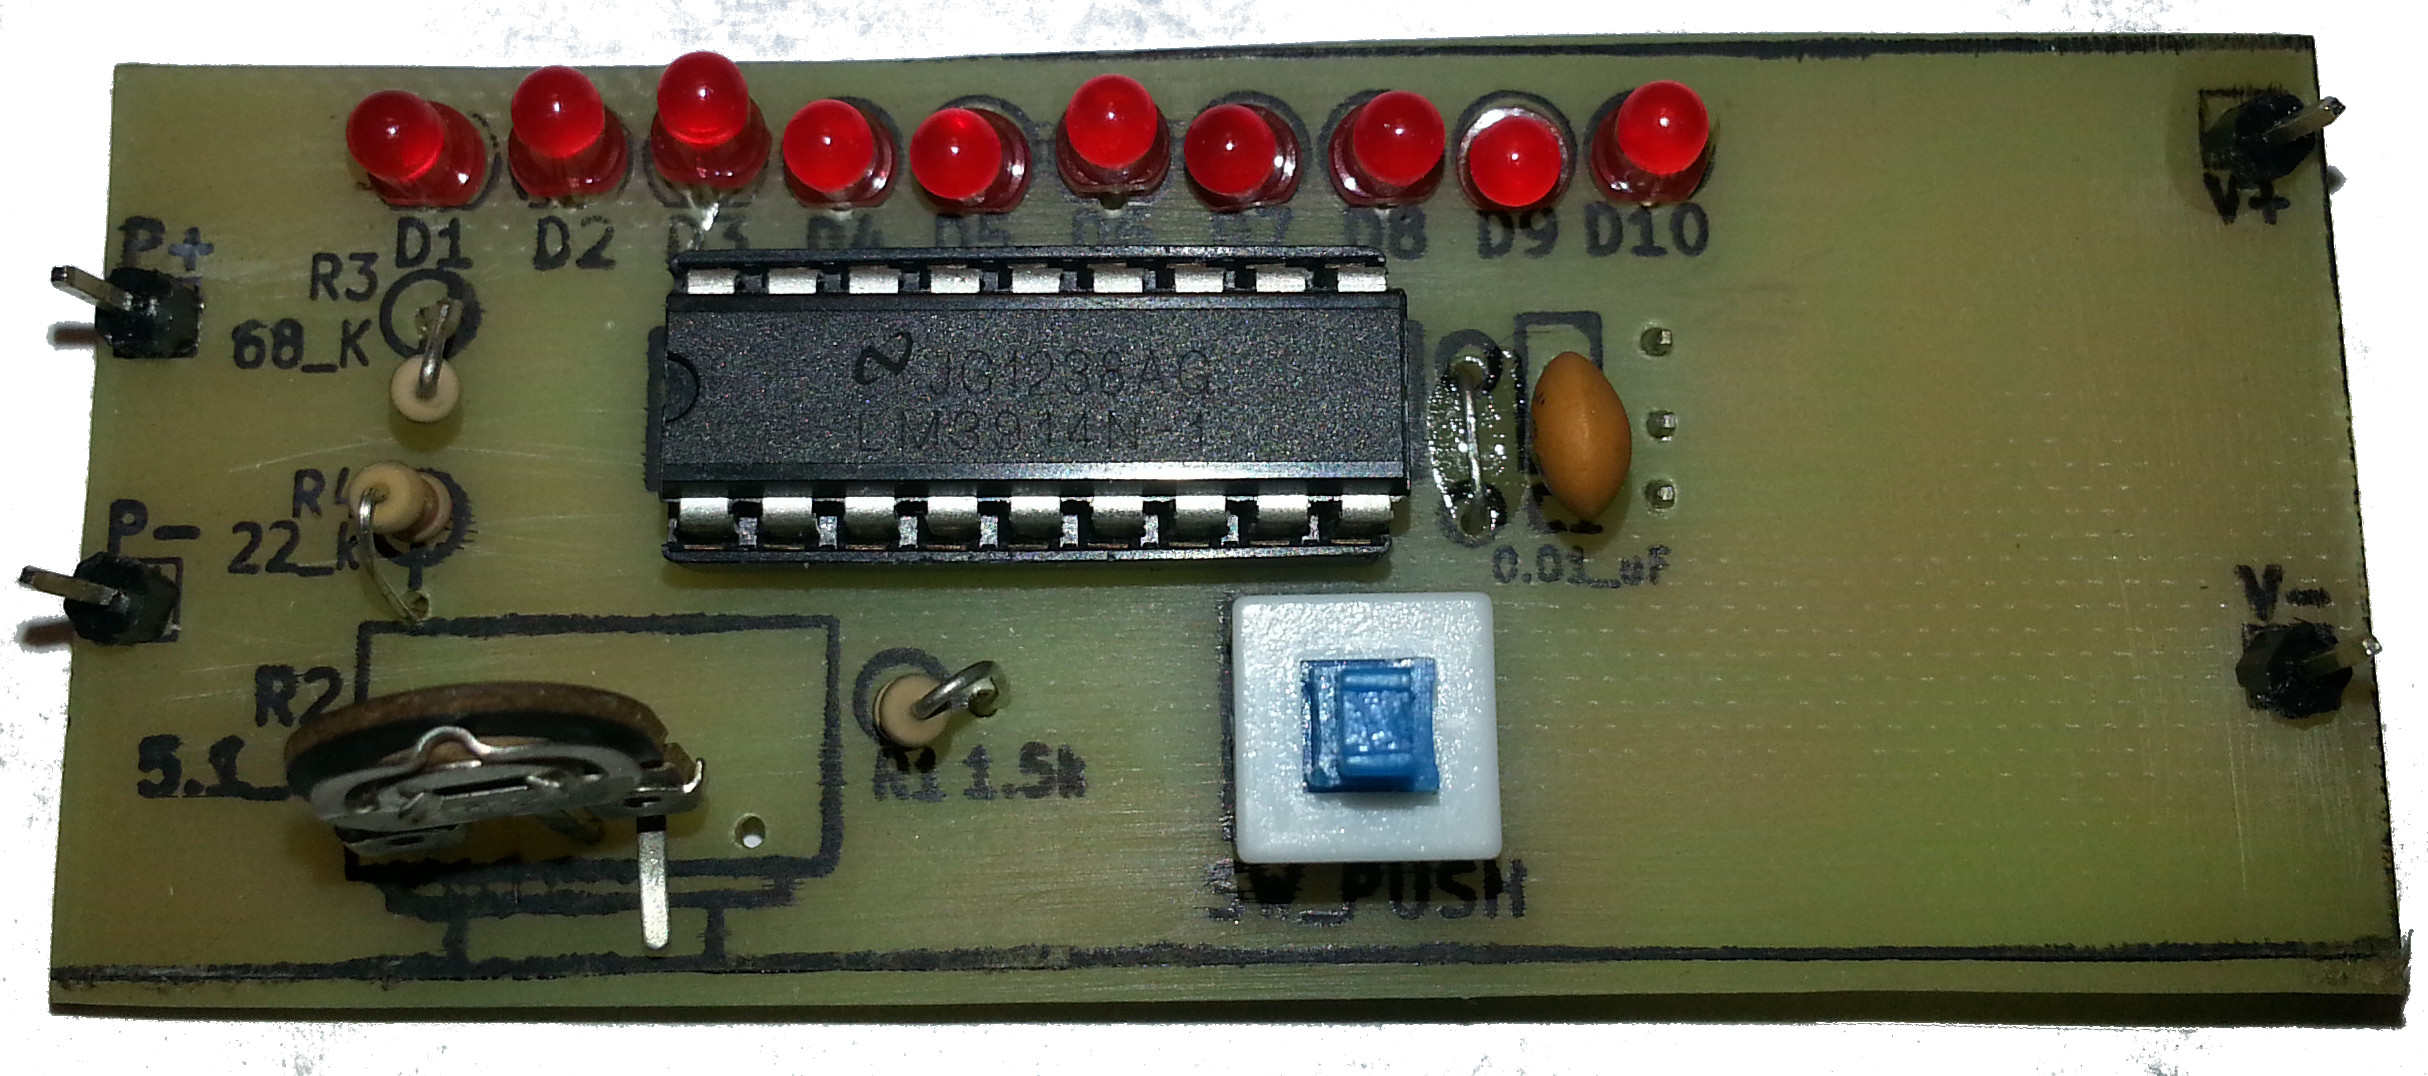
\includegraphics[scale=0.1]{images/placa_completa.jpg}\caption{Circuito Completo}
			\end{figure}

		\subsection{Materiales y Costo}

		\begin{center}
			
			{\footnotesize \begin{tabular}{ |c|l|r|r| }

			\hline
				\multicolumn{4}{|c|}{\textbf{Materiales}}\\ \hline
				Cantidad & Descripción & Precio Unitario [\$] & Subtotal [\$] \\ \hline
				1 & Resistor $1.5 \: k\Omega$ & $0.25$ & $0.25$\\ \hline
				1 & Resistor variable $10 \: k\Omega$ & $8$& $8$ \\ \hline
				1 & Resistor $68 \: k\Omega$ & $0.25$&$0.25$ \\ \hline
				1 & Resistor $22 \: k\Omega$ & $0.25$& $0.25$\\ \hline
				10 & LED Rojo 3 mm & $1.5$ & $15$\\ \hline
				1 & Capacitor Cerámico $0.01 \: \mu F$ & $1$& $1$\\ \hline
				1 & Pulsador 6 pines & $5$ & $5$ \\ \hline
				1 & Integrado LM3914 & $28$ & $28$\\ \hline
				1 & Regulador LM7812 & $5.5$& $5.5$ \\ \hline
				1 & Base Integrado 18 pines & $2$& $2$ \\ \hline
				1 & Placa Cobre 10x10 cm & $9$& $9$ \\ \hline
				1 & Hoja Transferencia Térmica & 10 & 10\\ \hline
				\multicolumn{4}{|r|}{Total:  $84.25$}\\ \hline


			\end{tabular}}\captionof{table}{Lista de Precios}\label{tab:costo}
			\end{center}

			\subsection{Cronograma de Trabajo}
				Se cumplió con el siguiente cronograma de trabajo, el mismo fue conforme a lo estipulado y a las limitaciones de carga horaria de la cursada.
				\begin{figure}[H]
					\centering
					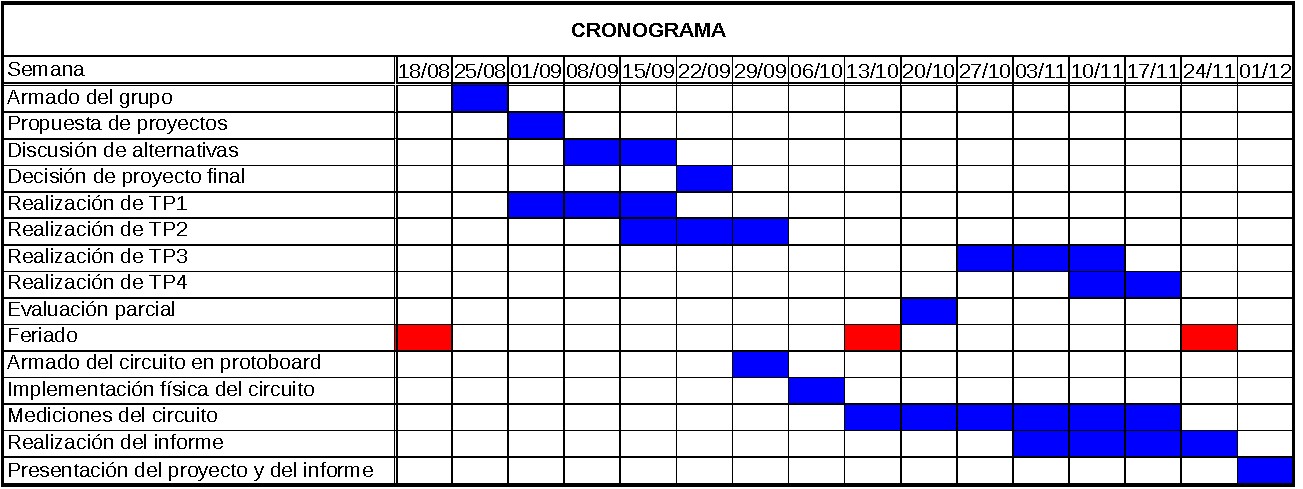
\includegraphics[scale=0.8]{images/Cronograma.pdf}\caption{Cronograma de Trabajo}
					\end{figure}

		\subsection{Mediciones}

			Siendo que para la realización de mediciones el circuito impreso no resulta muy apropiado por la dificultad (o imposibilidad) de conectar los terminales de los voltímetros se optó por emplear toda otra serie de compuestos en un \textit{protoboard} para así facilitar ciertas mediciones.

			\begin{figure}[H]
			\centering
				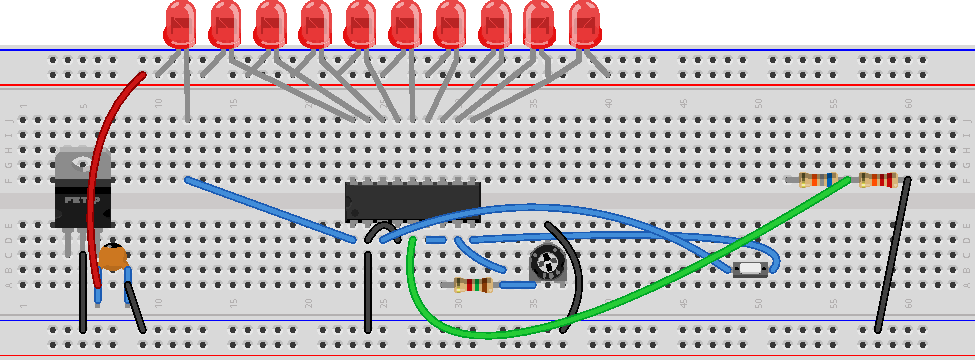
\includegraphics[scale=1]{images/proto.pdf}\caption{Protoboard}\label{fig:proto}
			\end{figure}

			Para todas las mediciones a realizar se empleará el multímetro digital MS8221A utilizado en los trabajos anteriores, en caso de emplearse otro se aclarará explícitamente. Asímismo las fuentes reguladas a utilizar serán las HY3005D empleadas con anterioridad, para el funcionamiento de este proyecto se emplearán dos, una como alimentación del circuito y otra como fuente a mensurar.

			\subsubsection{Regulador}

			Uno de los componentes claves del circuito es el regulador de tensión LM7812, el cual se emplea con el propósito de obtener una salida constante de 12 V. Como primera medición se mide la salida del regulador respecto de la entrada de tensión. Se espera que a bajos voltajes la tensión de salida sea similar a la tensión de entrada pero menor. Además se espera que la tensión para la cual la salida se estabiliza, este uno o dos voltios por encima de los 12 V.

			Empleando un simple banco de medición con una fuente y un voltímetro se obtuvieron los siguientes datos.

			\begin{figure}[H]
			\centering
				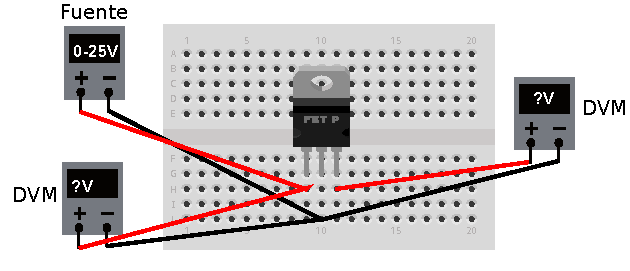
\includegraphics[scale=1]{images/reg.pdf}\caption{Banco de Medición Regulador de Tensión}\label{fig:banco0}
			\end{figure}

			\begin{center}
			{\footnotesize \begin{tabular}{ |l|l|l|l| }

			\hline
				\multicolumn{4}{|c|}{\textbf{Regulador Tensión}}\\ \hline
				$V_{in}$ & $\Delta V_{in}$ & $V_{out}$ & $\Delta V_{out}$ \\ \hline
				$1.62$ & $0.02$ & $0.97$ & $0.02$\\ \hline
				$3.24$ & $0.03$ & $2.55$ & $0.02$\\ \hline
				$4.96$ & $0.04$ & $4.2$ & $0.04$\\ \hline
				$7.56$ & $0.05$ & $6.75$ & $0.05$\\ \hline
				$10.34$ & $0.07$ &  $9.5$ & $0.05$\\ \hline
				$12.44$ & $0.08$ & $11.58$ & $0.07$\\ \hline
				$12.76$ & $0.08$ & $11.91$ & $0.07$\\ \hline
				$13$ & $0.08$ & $12.14$ & $0.08$\\ \hline
				$13.13$ & $0.08$ & $12.2$ & $0.08$\\ \hline
				$13.37$ & $0.08$ & $12.21$ & $0.08$\\ \hline
				$14.36$ & $0.09$ & $12.21$ & $0.08$\\ \hline
				$15.75$ & $0.09$ & $12.21$ & $0.08$ \\ \hline
				$17.38$ & $0.10$ & $12.22$ & $0.08$\\ \hline
				$20.1$ & $0.3$ &  $12.21$ & $0.08$ \\ \hline
				$22.4$ & $0.3$ &  $12.21$ & $0.08$ \\ \hline
				$24.5$ & $0.3$ &  $12.21$ & $0.08$ \\ \hline
				$28.1$ & $0.3$ &  $12.22$ & $0.08$ \\ \hline
				$31.4$ & $0.3$ &  $12.25$ & $0.08$ \\ \hline			
 				
				
			\end{tabular}}\captionof{table}{Medición LM7812}\label{tab:regtension}
			\end{center}

			Siendo $V_{in}$ la tensión de entrada al regulador y $V_{out}$ la de salida.

			\begin{figure}[H]
			\centering
				\includegraphics[scale=0.035]{images/med_reg.pdf}\caption{Tensión Salida Regulador}\label{fig:grafreg}
			\end{figure}

			Consistente con las hipótesis, la tensión de salida es lineal e inferior a la tensión de entrada a tensiones bajas. También se confirmo el punto en el cuál la tensión de salida se estabiliza (13.13 V) se encuentra por encima de la tensión de regulación. La figura \ref{fig:grafreg} no posee barras de errores dado a como es apreciable en el cuadro \ref{tab:regtension} los errores son despreciables respectos de los valores en los que se opera.

			Considerando la corriente de entrada del regulador\footnote{Ver sección \ref{sec:anexo}}  $8 \: mA$ la fuente se considera ideal considerándose dicha corriente baja, asimismo siendo la impedancia de salida del regulador $18 \: m\Omega$ muy inferior a la impedancia de entrada del mulímetro empleado ($10 \: M\Omega$) se considera que en ambas lecturas despreciable cualquier efecto de carga que pudiera existir. 

			\subsubsection{Escala}
				Acorde a las hipótesis realizadas, el vúmero posee un fondo de escala de 25 V distribuidos en 10 LEDs, por lo que cada LED representará un aumento en la tensión de 2,5 V. 

				\begin{center}
			{\footnotesize \begin{tabular}{ |c|l| }

			\hline
				\multicolumn{2}{|c|}{\textbf{Escala LEDs}}\\ \hline
				$\#$Led Encendido(s) & Tensión [V] \\ \hline
				$0$ & $< 2.5$ \\ \hline
				$1$ & $2.5$ \\ \hline
				$2$ & $5$ \\ \hline
				$3$ & $7.5$ \\ \hline
				$4$ & $10$ \\ \hline
				$5$ & $12.5$ \\ \hline
				$6$ & $15$ \\ \hline
				$7$ & $17.5$ \\ \hline
				$8$ & $20$ \\ \hline
				$9$ & $22.5$ \\ \hline
				$10$ & $25$ \\ \hline			
 				
				
			\end{tabular}}\captionof{table}{Escala leds}\label{tab:escala}
			\end{center}

			Para corrobororar esta escala y/o realizar los ajustes necesarios se emplearon dos fuentes reguladas, una como fuente de alimentación del circuito y otra como fuente a mensurar. Asimismo en paralelo con la fuente a mensurar se coloca un multímetro digital a fin de tener una lectura mas exacta de la tensión respecto de la mostrada por la pantalla LED de la fuente.

			\begin{figure}[H]
			\centering
				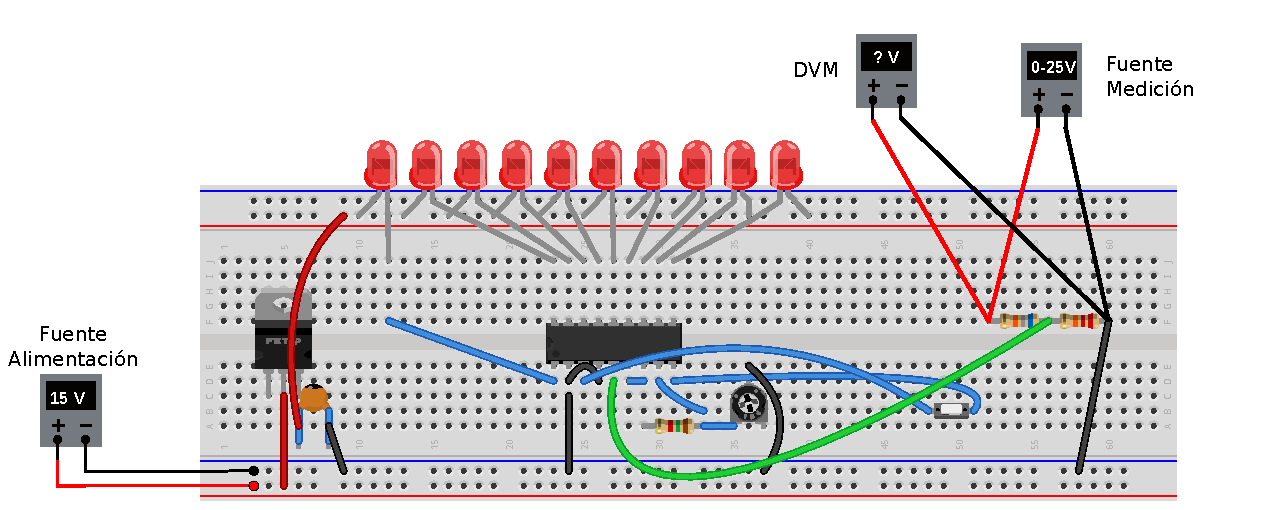
\includegraphics[scale=0.8]{images/banco1.pdf}\caption{Banco de Medición Escala}\label{fig:banco1}
			\end{figure}

			Con este banco de medición, se fue variando la tensión de salida de la fuente a mensurar corroborando que la secuencia de encendido de los leds sea consistente con el cuadro \ref{tab:escala}, al realizar esto fue evidente que la escala no estaba ajustada apropiadamente por lo que modificamos la resistencia del resistor variable hasta que nos de acorde a la escala previamente establecida. Como resultado, el nuevo valor

			\begin{equation}
				R_2 = (3.87 \pm 0.05) \: k \Omega
			\end{equation}

			Esta diferencia puede ser causada por diversas causas:
			\begin{itemize}
				\item Los resistores no son exactos, por lo cual pueden haber diferencias en su comportamiento respecto del modelo hipotético planteado.

				\item En los cálculos de las resistencias no se evalúa la posible alteración que produce el divisor de tensión (que ajusta el fondo de escala).


			\end{itemize}

			\textbf{Efecto de Carga:} Si bien se considera la lectura del DVM más exacta que la lectura del panel LCD de la fuente, al estar el multímetro conectado en paralelo con dos resistores de una resistencia conjunta de $90 \: k\Omega \cong 0.1 \: M\Omega$ de un orden inferior al de su resistencia interna de $10 \: M\Omega$ se considera el efecto mínimo.

			Una vez hecha esta modificación se planteó la necesidad de corroborar la escala sin utilizar la perilla de la fuente variable que consideramos poco precisa. Para ello se construyó un circuito de 10 resistores de $1 \: k\Omega$ en serie para usar como divisor de tensión, aplicando con la fuente variable una salida de tensión de 25 V.

			\begin{figure}[H]
			\centering
				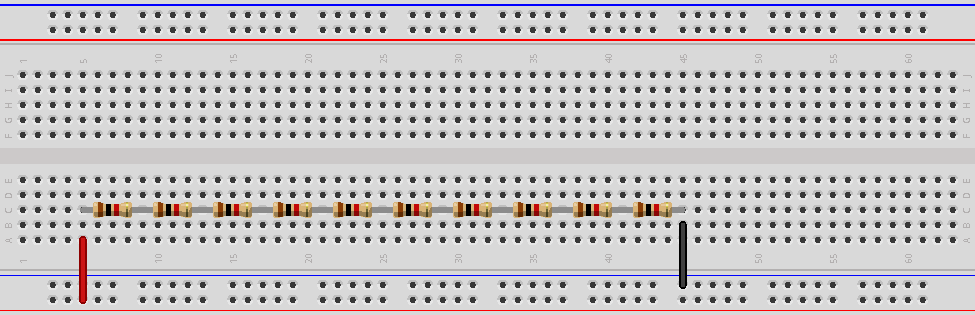
\includegraphics[scale=1]{images/div.pdf}\caption{Divisor de Tensión}\label{fig:divtens}
			\end{figure}

			De haber realizado correctamente los ajustes, el led que se enciende (o la cantidad depende el modo) debe corresponderse con los bornes que tomemos en el divisor de tensión. Por ejemplo en el siguiente banco no debe prenderse ningún led
			
			\begin{figure}[H]
			\centering
				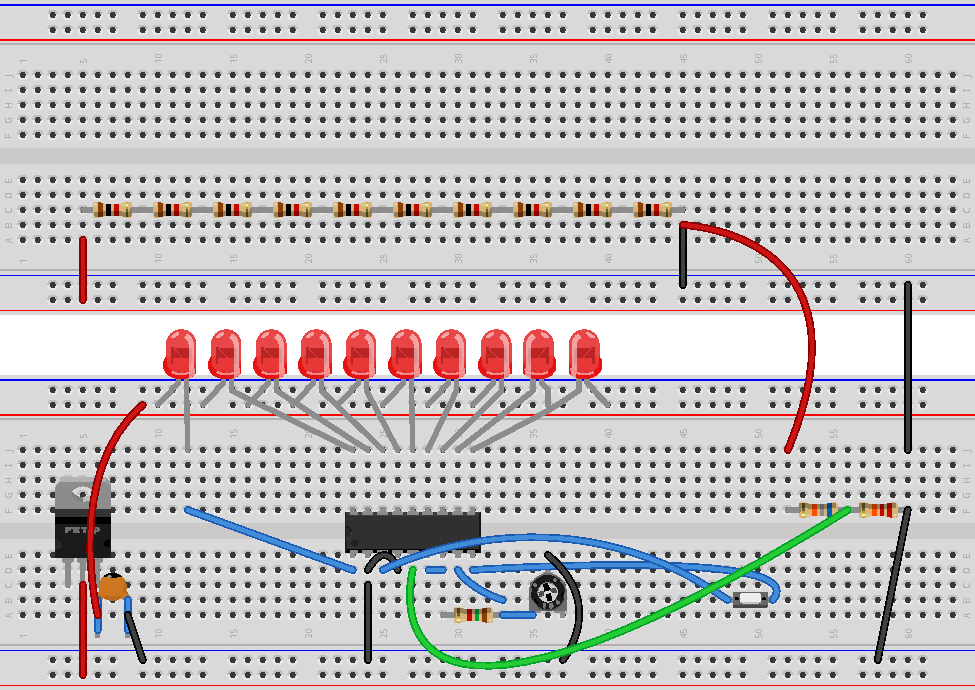
\includegraphics[scale=0.8]{images/labo1_bb3.pdf}\caption{Banco Medición Escala}
			\end{figure}

			\begin{figure}[H]
			\centering
				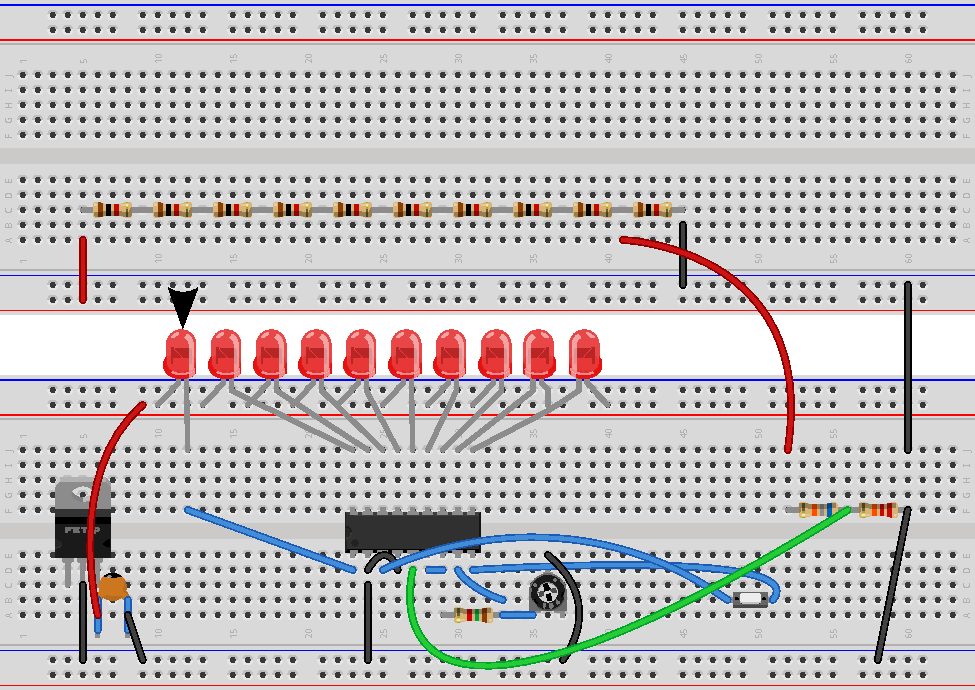
\includegraphics[scale=0.9]{images/labo1_bb2.pdf}\caption{Se enciende un led}
			\end{figure}

			\begin{figure}[H]
			\centering
				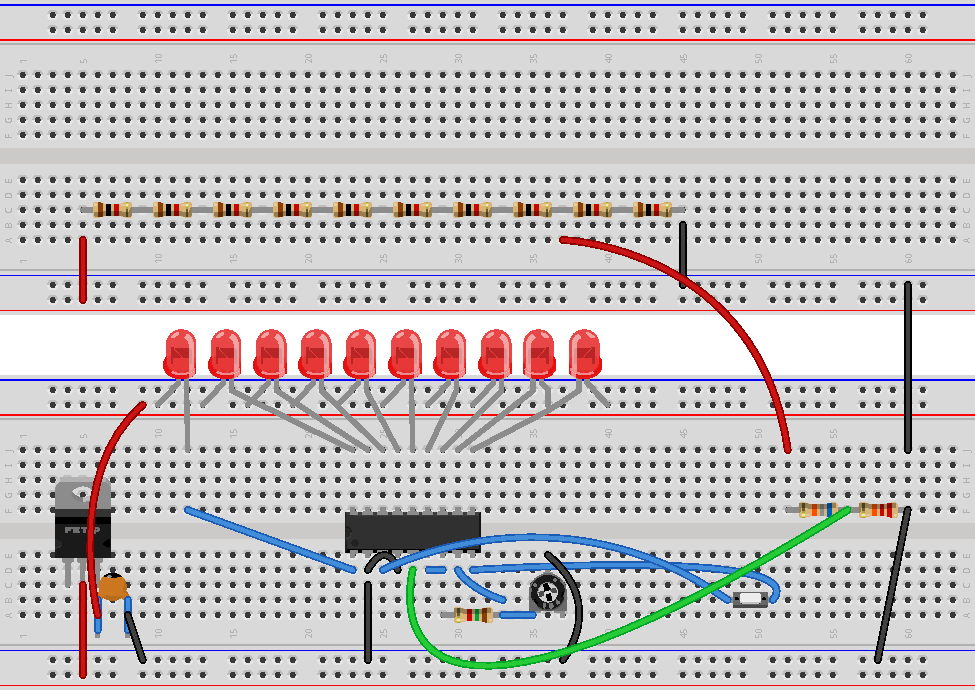
\includegraphics[scale=0.9]{images/labo1_bb1.pdf}\caption{Se encienden dos led}
			\end{figure}

			\begin{figure}[H]
			\centering
				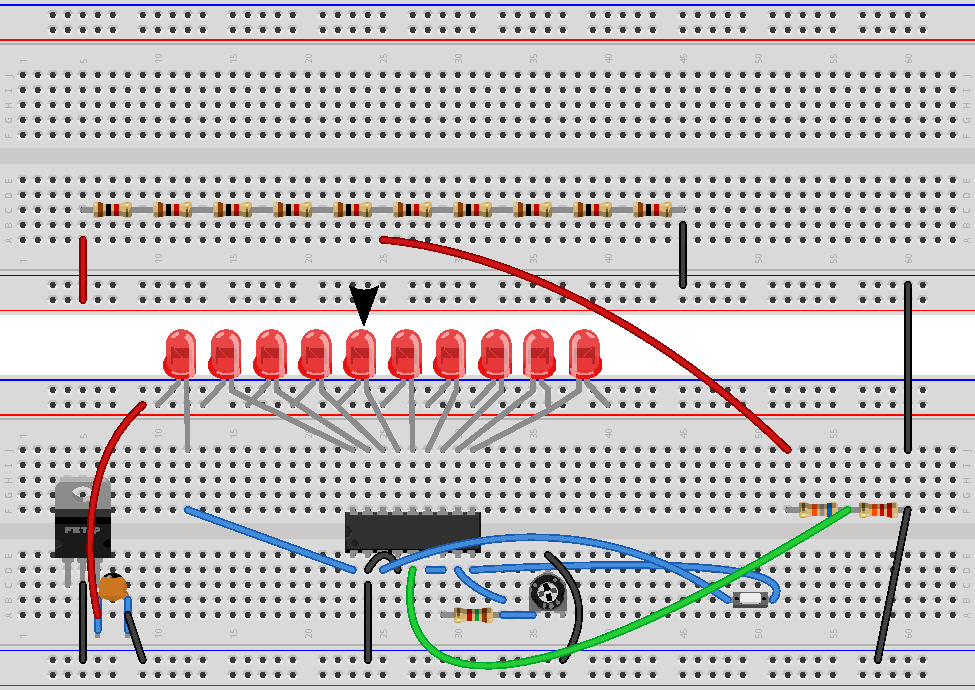
\includegraphics[scale=0.9]{images/labo1_bb.pdf}\caption{Se encienden cinco led}
			\end{figure}

			Al realizar estas pruebas, pudimos constatar que fehacientemente la escala era correcta.

			\begin{figure}[H]
			\centering
				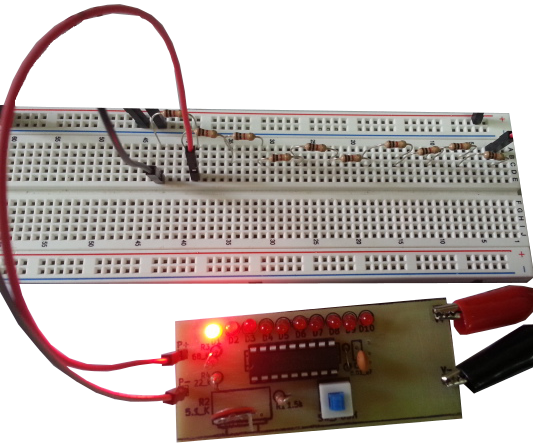
\includegraphics[scale=0.6]{images/res1.png}\caption{Prueba Encender un Led}
			\end{figure}

			\begin{figure}[H]
			\centering
				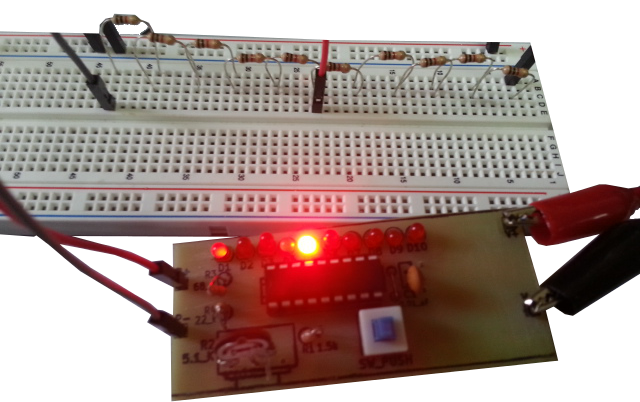
\includegraphics[scale=0.6]{images/res2.png}\caption{Prueba Encender cinco Led}
			\end{figure}

			\subsubsection{Corriente Led}

			Así como previamente verificamos que el resistor que establece el fondo de escala / paso del vúmetro sea de una resistencia correcta, otra de las interrogantes fue si el resistor $R_1$ que establece el paso de corriente hacia los LED era de un valor adecuado. Para ello utilizando el mismo banco de medición que con anterioridad, se puso un amperímetro en serie con alguno de los Leds y como resultado se obtuvo:

			\begin{equation}
				R_1 = (8.37 \pm 0.08) \: mA
			\end{equation}

			Este valor se obtuvo con el multímetro digital Sonel CMM-40 ya que el multímetro utilizado con anterioridad no tomaba bien la lectura. Asumimos que debido a que la tensión en los leds es muy baja al añadirle el instrumento este le agrega una impedancia que hace caer la corriente y por ende no tomar lectura. Otra posibilidad es que los multímetros MS8221A empleados al momento de esta medición tengan su modo amperímetro quemado.

			\begin{figure}[H]
			\centering
				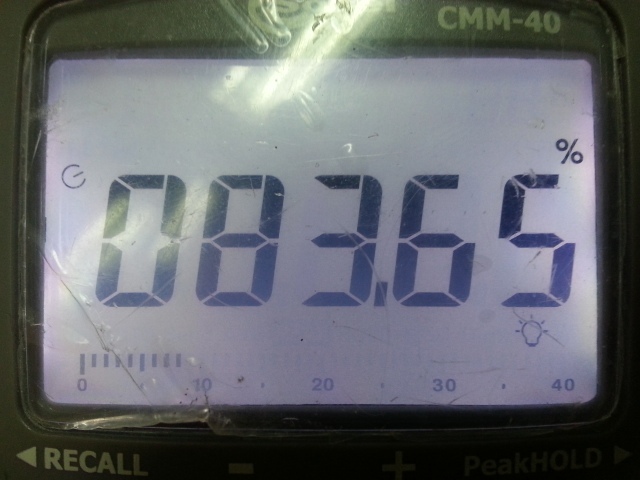
\includegraphics[scale=0.5]{images/sonel.jpg}\caption{Medición Corriente Led}
			\end{figure}

			Este resultado es consistente con lo hecho en el desarrollo previo del proyecto.

			\subsubsection{Consumo}
				Una de las principales características de este circuito, es la capacidad de cambiar entre modo BAR y modo DOT, obteniendo así una misma lectura expresada en un sólo led o en un continuo de leds. A priori se puede deducir que entre ambos modos habrá una diferencia de consumo proveniente de tener un sólo led o un número de leds. Asímismo se espera que en modo punto el consumo sea constante y lineal en modo barra, para ello se fue variando la tensión de la fuente a mensurar y se midió la corriente. Con dichos valores se calculó la potencia teniendo en cuenta que la tensión aplicada por la fuente de alimentación fue de 15 V.

				\begin{center}
			
			{\footnotesize \begin{tabular}{ |l|l|l|l|l|l| }

			\hline
				\multicolumn{6}{|c|}{\textbf{Mediciones DOT}}\\ \hline
				Tensión [V] & $\Delta V$ [V] & Corriente [mA] & $\Delta I$ [mA] & Consumo [mW] & $\Delta$ Consumo [mW]\\ \hline
				$0.40$ & $0.02$ & $10.2$ & $0.3$ & $153.0$ & $3.4$ \\ \hline
				$1.29$ & $0.02$ & $10.2$ & $0.3$ & $153.0$ & $3.4$ \\ \hline
				$2.50$ & $0.03$ & $24.3$ & $0.4$ & $364.5$ & $5.9$ \\ \hline
				$3.82$ & $0.03$ & $24.4$ & $0.4$ & $366.0$ & $5.9$ \\ \hline
				$5.08$ & $0.04$ & $24.3$ & $0.4$ & $364.5$ & $5.9$ \\ \hline
				$6.78$ & $0.05$ & $24.3$ & $0.4$ & $364.5$ & $5.9$ \\ \hline
				$7.50$ & $0.05$ & $23.7$ & $0.4$ & $355.5$ & $5.8$ \\ \hline
				$8.85$ & $0.06$ & $23.8$ & $0.4$ & $357.0$ & $5.8$ \\ \hline
				$10.61$ & $0.07$ & $24.5$ & $0.4$ & $367.5$ & $6.0$ \\ \hline
				$11.83$ & $0.07$ & $24.4$ & $0.4$ & $366.0$ & $5.9$ \\ \hline
				$12.64$ & $0.08$ & $24.4$ & $0.4$ & $366.0$ & $5.9$ \\ \hline
				$13.81$ & $0.08$ & $24.4$ & $0.4$ & $366.0$ & $5.9$ \\ \hline
				$15.08$ & $0.09$ & $24.1$ & $0.4$ & $361.5$ & $5.9$ \\ \hline
				$16.75$ & $0.1$ & $24.1$ & $0.4$ & $361.5$ & $5.9$ \\ \hline
				$17.63$ & $0.1$ & $24.0$ & $0.4$ & $360.0$ & $5.9$ \\ \hline
				$18.75$ & $0.1$ & $24.0$ & $0.4$ & $360.0$ & $5.9$ \\ \hline
				$20.0$ & $0.2$ & $23.7$ & $0.4$ & $355.5$ & $5.8$ \\ \hline
				$21.3$ & $0.2$ & $23.7$ & $0.4$ & $355.5$ & $5.8$ \\ \hline
				$22.5$ & $0.2$ & $23.9$ & $0.4$ & $358.5$ & $5.9$ \\ \hline
				$23.7$ & $0.2$ & $23.9$ & $0.4$ & $358.5$ & $5.9$ \\ \hline
				$25.0$ & $0.2$ & $24.0$ & $0.4$ & $360.0$ & $5.9$ \\ \hline
				$26.4$ & $0.2$ & $24.0$ & $0.4$ & $360.0$ & $5.9$ \\ \hline
 				
				
			\end{tabular}}\captionof{table}{Medición Consumo modo DOT}\label{tab:consumodot}
			\end{center}

			\begin{center}
			{\footnotesize \begin{tabular}{ |l|l|l|l|l|l| }

			\hline
				\multicolumn{6}{|c|}{\textbf{Mediciones BAR}}\\ \hline
				Tensión [V] & $\Delta V$ [V] & Corriente [mA] & $\Delta I$ [mA] & Consumo [mW] & $\Delta$ Consumo [mW]\\ \hline
				$0.40$  & $0.02$ & $ 10.3 $ &  $ 0.3 $ & $ 154.5$   & $ 6.4 $ \\ \hline
				$1.29$  & $0.02$ & $ 10.3$ &   $ 0.3 $ & $ 154.5$  & $ 6.4 $ \\ \hline
				$2.50$  & $0.03$ & $ 24.5 $ &  $ 0.4 $ & $ 367.5 $  & $ 9.0 $ \\ \hline
				$3.82$  & $0.03$ & $ 24.5 $ &  $ 0.4 $ & $ 367.5$  & $ 9.0 $ \\ \hline
				$5.08$  & $0.04$ & $ 38.5 $ &  $ 0.6 $ & $ 577.5 $ & $ 11.5 $ \\ \hline
				$6.78$  & $0.05$ & $ 38.5 $ &  $ 0.6 $ & $ 577.5 $ & $ 11.5$ \\ \hline
				$7.50$  & $0.05$ & $ 51.8 $ &  $ 0.8 $ & $ 777.0 $ & $ 13.9 $ \\ \hline
				$8.85$  & $0.06$ & $ 51.8 $ &  $ 0.8 $ & $ 777.0 $ & $ 13.9 $ \\ \hline
				$10.61$ & $0.07$ & $ 65.7 $ &  $ 0.9 $ & $ 985.5 $ & $ 16.4 $ \\ \hline
				$11.83$ & $0.07$ & $ 65.7 $ &  $ 0.9 $ & $ 985.5 $ & $ 16.4 $ \\ \hline
				$12.64$ & $0.08$ & $ 79.6 $ &  $ 1.1 $ & $ 1194.0 $ & $ 18.9 $ \\ \hline
				$13.81$ & $0.08$ & $ 79.6 $ &  $ 1.1 $ & $ 1194.0 $ & $ 18.9 $ \\ \hline
				$15.08$ & $0.09$ & $ 93.4$ &   $ 1.3 $ & $ 1401.0$ & $ 21.4 $ \\ \hline
				$16.75$ & $0.1$  & $ 93.4 $ &  $ 1.3 $ & $ 1401.0 $ & $ 21.4 $ \\ \hline
				$17.63$ & $0.1$  & $ 107.3 $ & $ 1.4 $ & $ 1609.5 $ & $ 23.9 $ \\ \hline
				$18.75$ & $0.1$  & $ 107.3 $ & $ 1.4 $ & $ 1609.5 $ & $ 23.9 $ \\ \hline
				$20.0$  & $0.2$  & $ 120.4 $ & $ 1.6 $ & $ 1806.0 $ & $ 26.2 $ \\ \hline
				$21.3$  & $0.2$  & $ 120.5 $ & $ 1.6 $ & $ 1807.5 $ & $ 26.2 $ \\ \hline
				$22.5$  & $0.2$  & $ 133.0 $ & $ 1.7 $ & $ 1995.0 $ & $ 28.5 $ \\ \hline
				$23.7$  & $0.2$  & $ 133.1 $ & $ 1.7 $ & $ 1996.5 $ & $ 28.5 $ \\ \hline
				$25.0$  & $0.2$  & $ 145.0 $ & $ 1.9 $ & $ 2175.0 $ & $ 30.7 $ \\ \hline
				$26.4$  & $0.2$  & $ 145.2 $ & $ 1.9 $ & $ 2178.0 $ & $ 30.7 $ \\ \hline
 				
				
			\end{tabular}}\captionof{table}{Medición Consumo modo BAR}\label{tab:consumobar}
			\end{center}

			Con toda esta información disponible, es posile comparar mediante gráficos y confirmar algunas deducciones.

			\begin{figure}[H]
			\centering
				\includegraphics[scale=0.03]{images/corriente.pdf}\caption{Corriente vs Tensión}\label{fig:corriente}
			\end{figure}

			Como era de esperarse, la corriente en modo punto es constante observándose sólo un salto siendo que antes de los $2.5 \:V$ no se encuentra ningun led encendido. Asimismo se observa que en modo bar la corriente es lineal, habiendo unos descansos correspondientes a tensiones dentro del rango de un mismo led. 

			Una interrogante que se puede desprender de este gráfico es si dichos saltos son constantes.

			\begin{figure}[H]
			\centering
				\includegraphics[scale=0.03]{images/salto.pdf}\caption{Saltos Corriente}
			\end{figure}

			Estos saltos corresponden al valor de una corriente respecto de la corriente antes mensurada. Otra vez es observable como en modo punto sólo hay un salto y luego los saltos se encuentran muy próximos a 0. Para el modo bar, se observa una oscilacion correspondiente a que los puntos dentro del mismo rango de tension de un led (eg: 2,6 V y 3.0 V encienden el mismo led) no hay salto de corriente significativo, pero al encender un nuevo led si. Asimismo es visible como los valores pico de estos saltos se mantienen dentro de un rango discreto.

			\begin{figure}[H]
			\centering
				\includegraphics[scale=0.03]{images/pot.pdf}\caption{Potencia}\label{fig:potencia}
			\end{figure}

			Es observable como la potencia disipada por el circuito en modo BAR no sólo es mayor al de modo DOT punto a punto, sino también describe una progresión lineal lo cual es consistente con las hipótesis planteadas de que este crecimiento corresponde al encendido sucesivo de leds.

			\textbf{Efecto de Carga:} Utilizándose los multímetros en modo amperímetro, se considera su impedancia de entrada como mínima para evitar interacción con el circuito y por ello el efecto de carga despreciable.

		\subsection{Especificaciones}
			\begin{center}
			
			{\footnotesize \begin{tabular}{ |l|l|l|l|c| }

			\hline
			Especificación & Valor Esperado & Valor Mensurado & Corrimiento & Cumplido \\ \hline
			Salida Estable Regulador & $12 \: V$ & $12.21 \: V$ & $0.21 \: V$ &  \cellcolor{green!100} SI \\ \hline
			Entrada Minima para Estabilidad & $ 14.6 \: V$ & $13.13 \:V$ & $1.47 \:$ & \cellcolor{green!100} SI \\ \hline
			Escala Led & $2.5 \:V$ & $2.5 \: V$ & $0 \:V$ &\cellcolor{yellow!100} SI \\ \hline
			Corriente Led & $8.3 \: mA$ & $8.37 \: mA$ & $0.03 \: mA$ & \cellcolor{green!100} SI \\ \hline
			Corriente Maxima sin leds prendidos (DOT/BAR) & $12.2 \: mA$ & $10.3 \: mA$ & $1.9 \: mA$ & \cellcolor{green!100} SI \\ \hline
			Corriente Maxima (DOT) & $25.2 \: mA$ & $24.5 \: mA$ & $0.7 \: mA$ & \cellcolor{green!100} SI \\ \hline
			Corriente Maxima (BAR) & $142.2 \: mA$ & $145.2 \: mA$ & $3 \: mA$ & \cellcolor{yellow!100} SI \\ \hline
							
				
			\end{tabular}}\captionof{table}{Especificaciones}\label{tab:specs}
			\end{center}

		Los resultados resaltados en amarillo se consideran cumplidos habiendo notas adicionales a hacer en cada uno de ellos, verde se considera cumplido y rojo no cumplido. 
		\begin{itemize}
			\item \textbf{Entrada Minima para Estabilidad:} Si bien las mediciones arrojaron un valor menor al especificado, esto es coherente con la necesidad del fabricante de mantener un margen de seguridad para sus especificaciones como se ha visto en TPs anteriores.
			\item \textbf{Escala Led:} Si bien en un principio no se cumplió la especificación, se realizaron las modificaciones necesarias.
			\item \textbf{Corriente Máxima (BAR)}: Para el cálculo del valor esperado sólo se consideró el consumo del regulador de tensión, integrado y led, por lo que un leve corrimiento respecto de la medición es esperable. 
		\end{itemize}

	\newpage\null\thispagestyle{empty}\newpage
	
	\section{Escalabilidad}	\label{sec:escalabilidad}

		Pensando en las aplicaciones prácticas de un voltímetro, nos encontramos con la necesidad de poder obtener una lectura exacta y/o a distancia. Un vúmetro si bien es de lectura sencilla, no nos da un valor númerico ni tampoco nos permite leer la lectura a distancia. Si pensamos esto a nivel industrial es una gran desventaja, quizá por cuestiones de la complejidad de un determinado proceso es preciso obtener una lectura exacta; asimismo las extensiones de las plantas industriales obligan a realizar mediciones mediante sensores que reporten a una base central, para consultarlas en un centro de control.

		Abstrayendonos del caso insdustrial planteado y aprovechando que un compañero poseía un Arduino y Raspberry, decidimos implementar un voltímetro que muestre en una pantalla LED la tensión mensurada y asímismo permita una lectura a distancia. Para ello utilizamos un Arduino Mega 2560 R3 \footnote{\url{http://arduino.cc/en/Main/arduinoBoardMega} } con un \textit{shield} LCD DFRobot\footnote{\url{http://www.dfrobot.com/wiki/index.php?title=Arduino_LCD_KeyPad_Shield_(SKU:_DFR0009)} } y una Raspberry Pi B+ \footnote{\url{http://www.raspberrypi.org/products/model-b-plus/} }.

		En nuestro caso el Arduino actuará como sensor, que no sólo tomará las mediciones y las mostrará en una pantalla LCD sino que también las comunicará a la Raspberry por puerto serie. La Raspberry representará un sistema central de obtención de mediciones, en la misma se instaló un servidor web Apache y una simple página en PHP que muestra vía web las tensiones mensuradas en tiempo real. Además esta configuración nos permitiría registrar un historial de las mediciones realizadas para posterior análisis.

		Utilizando el mismo rango de tensiones utilizado con el vúmetro y siendo la máxima tensión permitida por el Arduino de 5 V es necesario utilizar un resistor de tensión, para lo cuál se utilizaron resistores de $100 \: \Omega$ y $1 \: k\Omega$. 

		\begin{figure}[H]
			\centering
				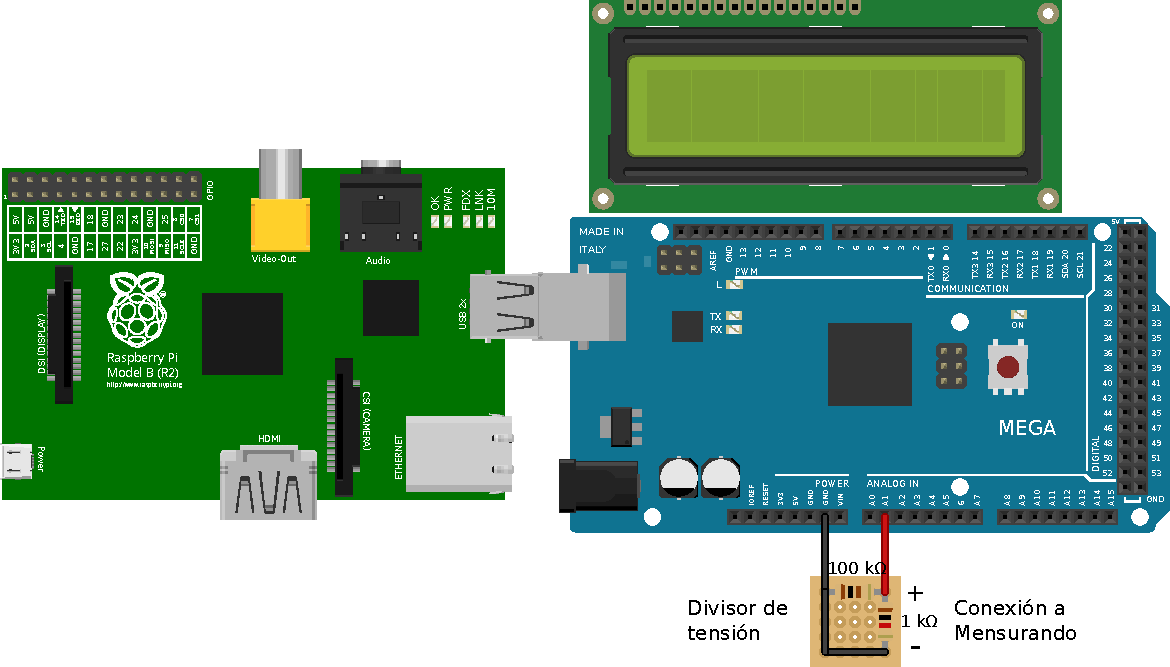
\includegraphics[scale=0.8]{images/arduino1.pdf}\caption{Banco Medición Arduino - Raspberry}
			\end{figure}

		Mediante un software compilado y cargado previamente, el Arduino mide la tensión aplicada al puerto analógico indicado (en este caso A1), calcula la tensión de la fuente mensurada teniendo en cuenta las características del resistor de tensión e imprime en el LCD el valor además de transmitirlo por puerto serie (emulado por USB). La pantalla LCD muestra el voltaje medido por el sensor y la tensión calculada.

		\begin{figure}[H]
			\centering
				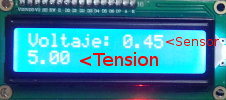
\includegraphics[scale=1.5]{images/ard1.png}\caption{Prueba LCD}
			\end{figure}

			\begin{figure}[H]
			\centering
				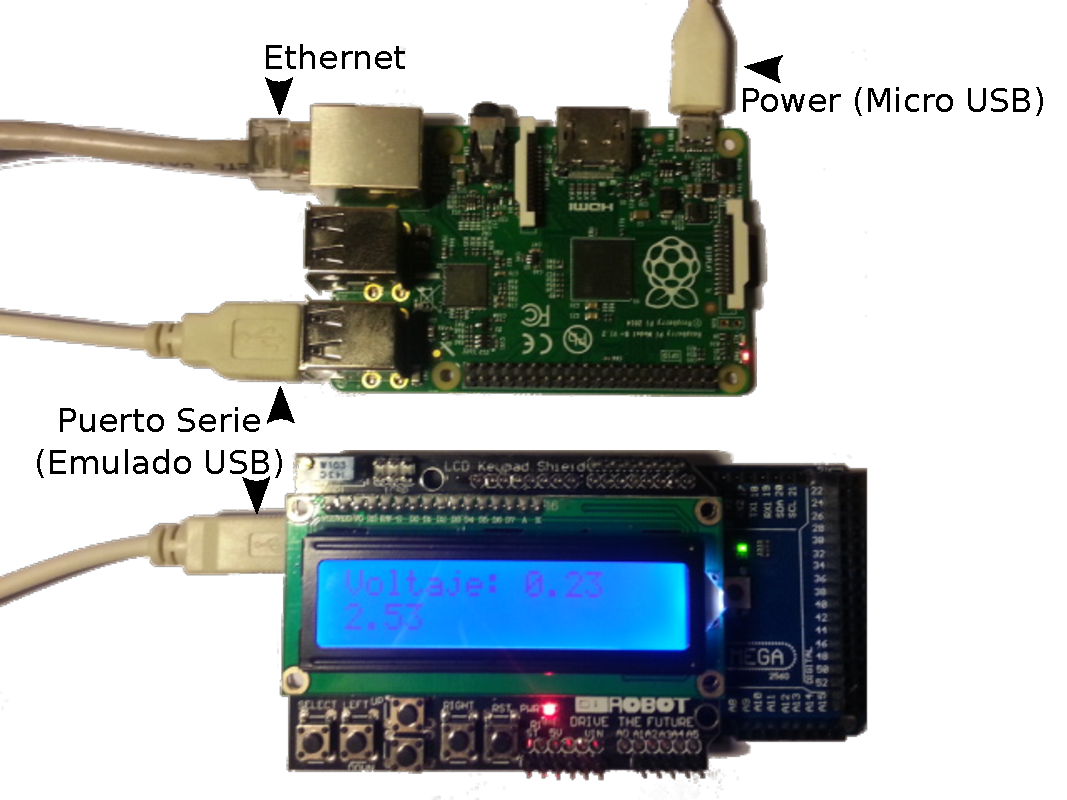
\includegraphics[scale=0.75]{images/arduino7.pdf}\caption{Conexión Arduino - Raspberry}
			\end{figure}

			\begin{figure}[H]
			\centering
				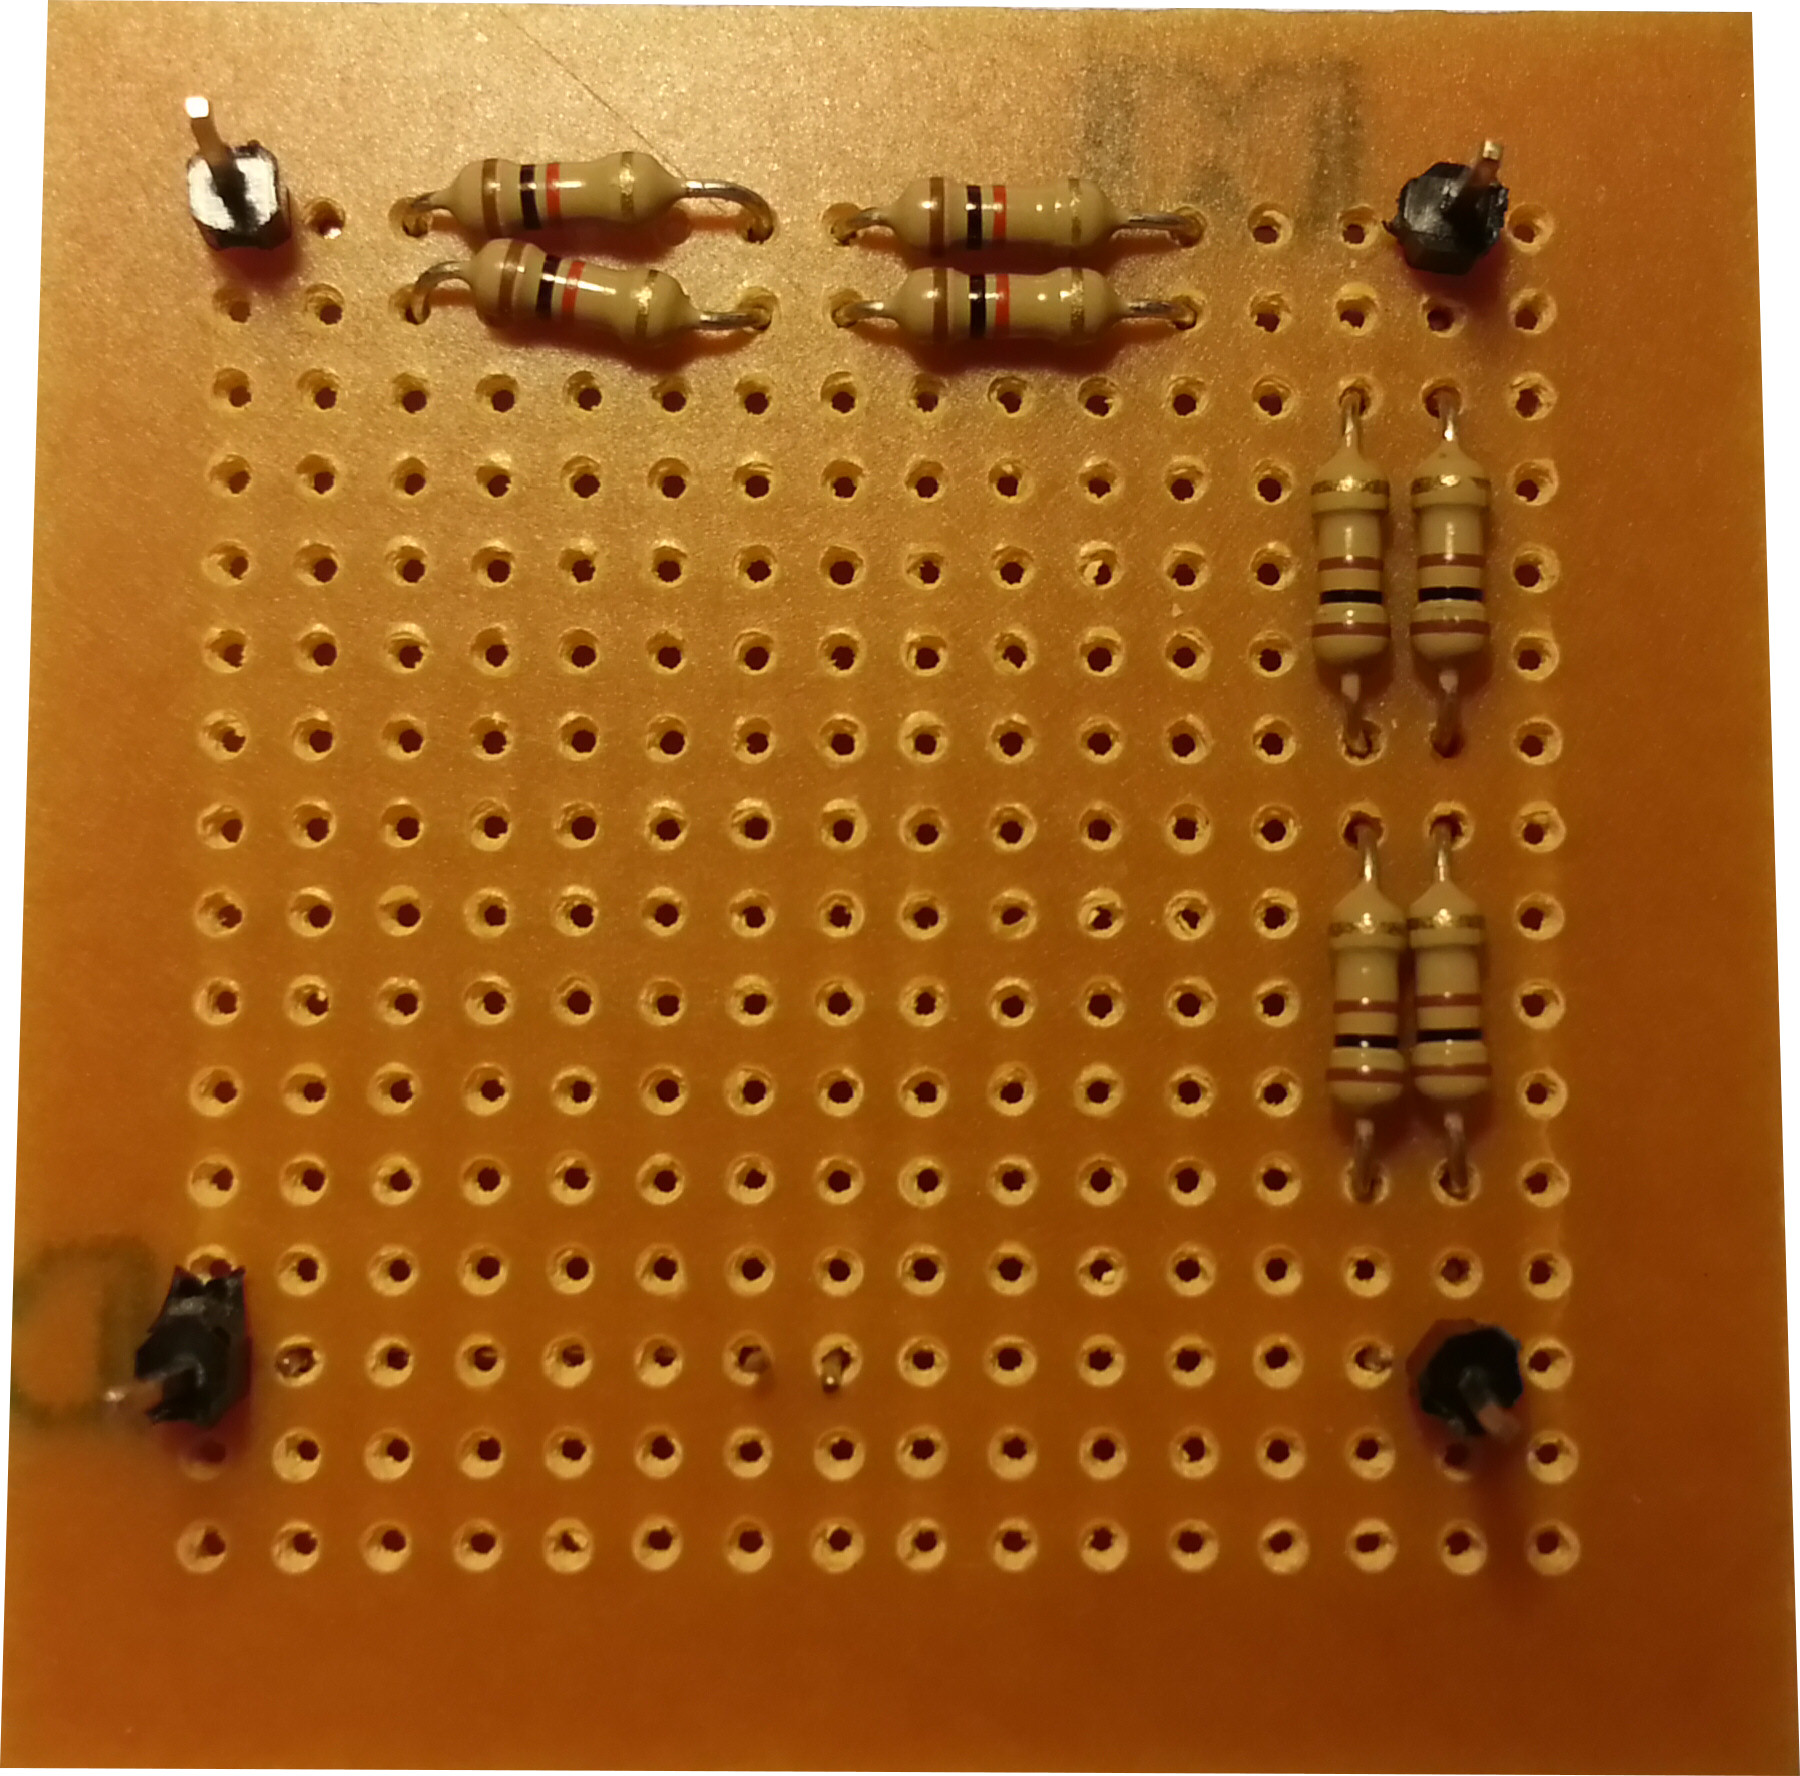
\includegraphics[scale=0.1]{images/div.jpg}\caption{Divisor Tensión Empleado}
			\end{figure}

		\subsection{Funcionalidades}\label{sec:func}

			A continuación se explicará brevemente las funcionalidades del esquema armado

			\begin{itemize}
				\item \textbf{Simple Visualización:} La pantalla led permite una lectura rápida y exacta de la tensión medida.
				\item \textbf{Comandos Locales:} Si bien no estan implementados, la pantalla LCD posee unos botones que podría permitirnos cambiar el comportamiento del lector. Un ejemplo posible es medir mas de una tensión e ir cambiando cuál de ellas mostrar en pantalla.
				\item \textbf{Comandos a Distancia:} Así como el Arduino envía datos por puerto Serie hacia la Raspberry, es capaz de recibirlos.
				\item \textbf{Lecturas a Distancia:} La Raspberry posee un servidor web Apache, que nos permite acceder a las lecturas via intra o internet.
				\item \textbf{Registros:} Cada lectura se guarda en un archivo con un timestamp en formato CSV, lo que nos permitiría a futuro efectuar un análisis de estos datos, graficarlos, calcular histogramas, etc.
			\end{itemize}

		\subsection{Materiales y Costo}

			\begin{center}
			
			{\footnotesize \begin{tabular}{ |l|l| }

			\hline
				\multicolumn{2}{|c|}{\textbf{Materiales}}\\ \hline
				Descripción & Precio[\$] \\ \hline
				Arduino Mega 2560 R3 & $399.90$ \\ \hline
				Arduino LCD DFRobot Shield & $179.90$ \\ \hline
				Raspberry Pi B+ & $989.90$ \\ \hline

				\multicolumn{2}{|r|}{Total:  $1569.7$}\\ \hline


			\end{tabular}}\captionof{table}{Lista de Precios}\label{tab:costo2}
			\end{center}

			Si bien el costo es elevado, ya disponiamos de los elementos. Además hay que tener en cuenta que son reutilizables para otros proyectos y que cumplen la función de prototipo, por lo que es posible conseguir un producto con las mismas capacidades afines a este proyecto, a costos más bajos.

		\subsection{Demo}

			En esta sección de mostrará brevemente en imágenes el funcionamiento general del artefacto y sus funcionalidades.

			La Raspberry al estar conectada en red, nos permite conectarnos a la \textit{shell} de Linux mediante SSH.

			\begin{figure}[H]
			\centering
				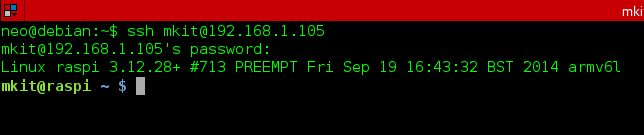
\includegraphics[scale=0.7]{images/Screenshot1.png}\caption{Acceso SSH}
			\end{figure}

			De esta manera podriamos tanto acceder a las lecturas como modificar los programas que las obtienen/muestran. Una vez en la \textit{shell}, se ejecuta un programa escrito en Python que es el encargado de abrir el puerto serie, imprimir las lecturas y guardarlas en los archivos correspondientes.

			\begin{figure}[H]
			\centering
				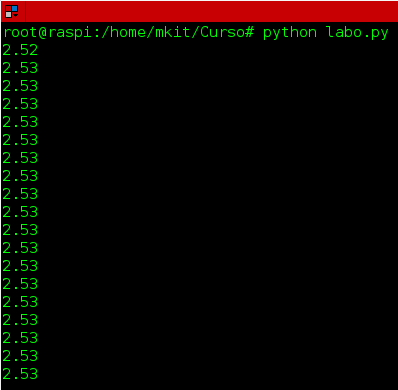
\includegraphics[scale=0.7]{images/Screenshot2.png}\caption{Ejecución Script}
			\end{figure}

			Como es visible, el programa muestra por pantalla las lecturas que se van comunicando por puerto Serie. Estas mismas además se guardan en un archivo de logs, junto con un timestamp en formato CSV. Este es útil si deseamos hacer un análisis a posteriori de las lecturas.

			\begin{figure}[H]
			\centering
				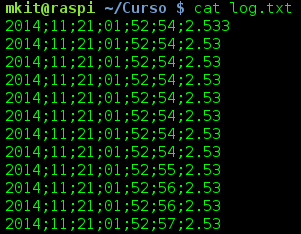
\includegraphics[scale=0.7]{images/Screenshot3.png}\caption{Log CSV con fecha y hora}
			\end{figure}

			Estas mismas lecturas son guardadas en un archivo que sirve de intermediario entre el script en Python y una página escrita en PHP, que lee dicho archivo y muestra en una web la última lectura realizada. La página está configurada para cada 500 ms volver a leer el archivo y así obtener una lectura en "tiempo real".

			\begin{figure}[H]
			\centering
				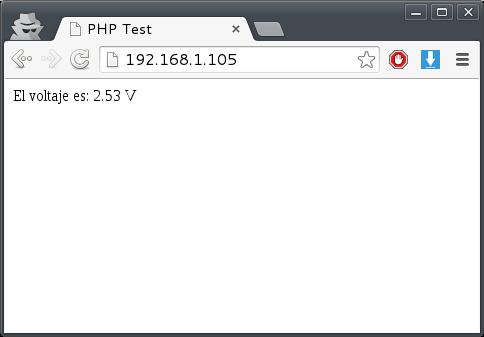
\includegraphics[scale=0.7]{images/Screenshot4.png}\caption{Vista WEB}
			\end{figure}

			\subsubsection{Graficador en Vivo}
				Como prueba de concepto, se escribió un programa en Python el cuál toma la comuniación en puerto serie y mediante la librería gráfica MatPlotLib \footnote{\url{http://matplotlib.org/}} grafica y actualiza la gráfica a medida que van llegando lecturas mediante el puerto serial. Para ello se armó un banco de prueba con la entrada analógica del arduino A1 con la posibilidad de conectarla a las salidas de 3.3 V, 5 V y GND del Arduino.

				\begin{figure}[H]
					\centering
					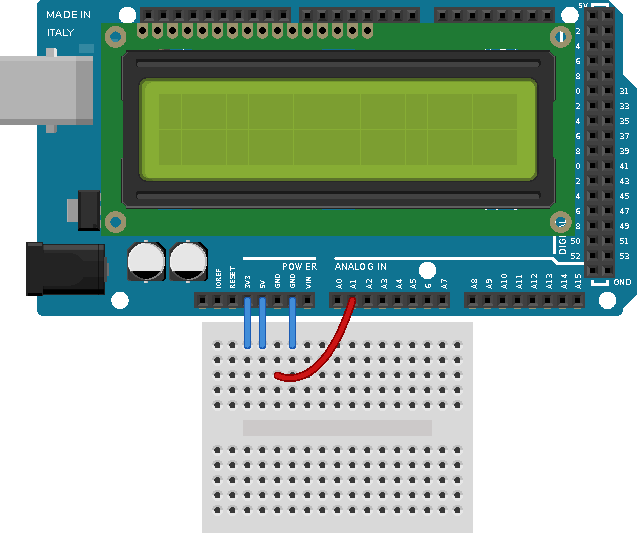
\includegraphics[scale=1]{images/arduino8.pdf}\caption{Banco de Prueba}
					\end{figure}

				\begin{figure}[H]
					\centering
					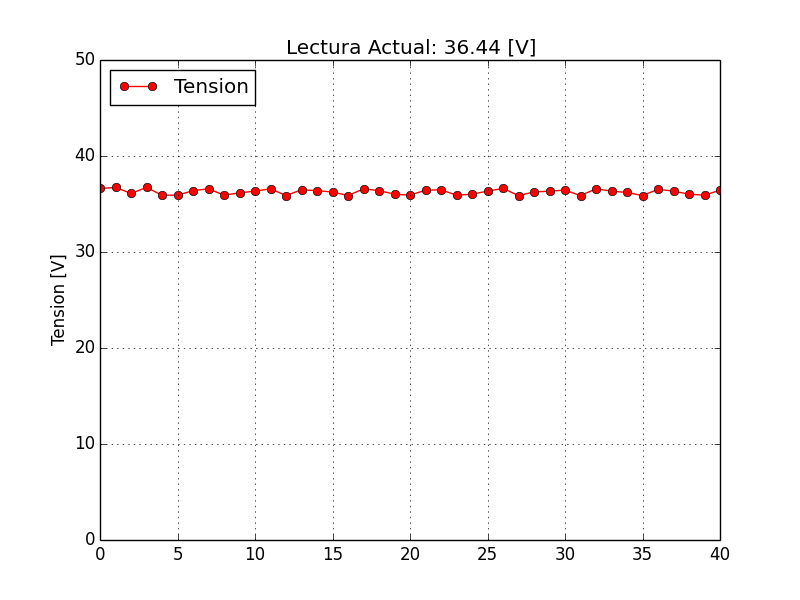
\includegraphics[scale=0.75]{images/figure_1.png}\caption{Captura de Gráfica}
					\end{figure}

				Con motivo de poder apreciarse la animación del gráfico, se grabó un video y se subió a YouTube en el cuál se muestra la pantalla del Arduino y la gráfica que muestra las lecturas al mismo tiempo. El link al video es \url{http://youtu.be/Gr6E5Hn9Tg4}.

			\subsubsection{Análisis de Datos}
				Haciendo uso del archivo CSV, podemos importar los datos a una planilla de cálculo de manera sencilla para operar con los mismos. En este caso importamos una serie de 100 mediciones en una planilla de LibreOffice Calc \footnote{\url{http://www.libreoffice.org/}} y con ellos calculamos los valores mínimo, máximo y promedio de las tensiones medidas. Tanto el archivo CSV como la planilla de cálculos se encuentran disponibles en el repositorio git \footnote{Ver sección \ref{sec:referencias}}.

				\begin{figure}[H]
					\centering
					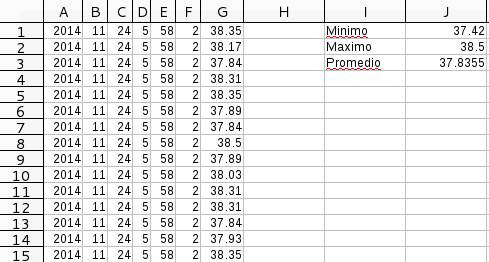
\includegraphics[scale=1]{images/arduino9.png}\caption{Hoja de Cálculos}
					\end{figure}

				Utilizando la misma planilla de cálculos podemos graficar los datos y obtener una imagen del valor promedio

				\begin{figure}[H]
					\centering
					\includegraphics[scale=0.03]{images/arduino10.pdf}\caption{Gráfico CSV}
					\end{figure}


		\subsection{Mediciones}

			Dada la premisa de esta escalabilidad la exactitud, una de las primeras cosas a mensurar fue cuán exacta es la medición del artefacto armado. Para ello se armó un banco de medición con un multímetro digital, considerándose la lectura de éste como exacta y contrastando las lecturas del Arduino con ellas.

			\begin{figure}[H]
			\centering
				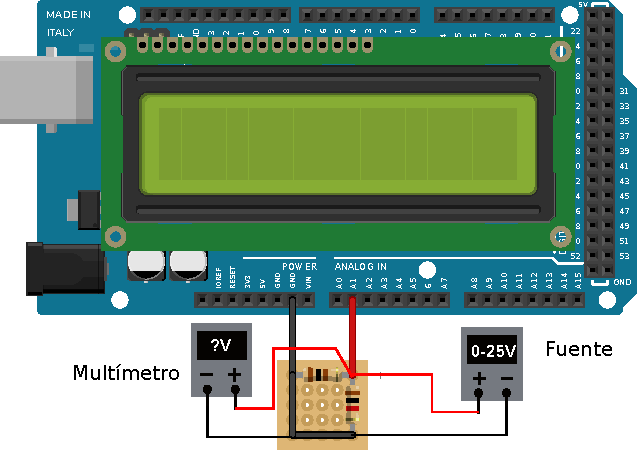
\includegraphics[scale=1.2]{images/arduino2.pdf}\caption{Banco de Medición Arduino}
			\end{figure}

			Como datos a evaluar se consideró la tensión de salida de la fuente, la tensión de salida del divisor de tensión calculada analíticamente, la lectura del sensor y la lectura calculada por el arduino.

			\begin{center}
			{\footnotesize \begin{tabular}{ |l|l|l|l|l|l| }

			\hline
				\multicolumn{6}{|c|}{\textbf{Mediciones Arduino}}\\ \hline
				$V_{fuente}$ [V]& $V_{divisor}$ [V]& $V_{sensor}$ [V]& $ V_{lectura}$ [V]& $| V_l - V_f |$ [V]& $\epsilon _r$\\ \hline
				$ 2.65  $ & $0.24$ & $0.23$ & $2.53  $ & $ 0.12  $  & $  0.05 $\\ \hline                                                                 
				$ 5.06  $ & $0.46$ & $0.45$ & $4.92  $ & $ 0.14  $  & $  0.03 $\\ \hline                                                                 
				$ 7.3   $ & $0.66$ & $0.65$ & $7.17  $ & $ 0.13  $  & $  0.02 $\\ \hline                                                                
				$ 9.17  $ & $0.83$ & $0.81$ & $8.98  $ & $ 0.19  $  & $  0.02 $\\ \hline                                                                 
				$ 12.21 $ & $1.10$ & $1.09$ & $11.97 $ & $ 0.15  $  & $  0.01 $\\ \hline                                                                   
				$ 13.51 $ & $1.23$ & $1.21$ & $13.32 $ & $ 0.19  $  & $  0.01 $\\ \hline                                                                  
				$ 15.16 $ & $1.38$ & $1.36$ & $14.97 $ & $ 0.19  $  & $  0.01 $\\ \hline                                                                  
				$ 17.42 $ & $1.58$ & $1.57$ & $17.26 $ & $ 0.16  $  & $  0.01 $\\ \hline                                                                  
				$ 18.38 $ & $1.67$ & $1.74$ & $19.22 $ & $ 0.84  $  & $  0.05 $\\ \hline                                                                  
				$ 21.7  $ & $1.97$ & $1.96$ & $21.66 $ & $ 0.04  $  & $  0.00 $\\ \hline                                                                   
				$ 22.8  $ & $2.07$ & $2.07$ & $22.7  $ & $ 0.10  $  & $  0.00 $\\ \hline                                                                 
				$ 24    $ & $2.18$ & $2.17$ & $24.0  $ & $ 0.00  $  & $  0.00 $\\ \hline                                                                 
				$ 25.3  $ & $2.30$ & $2.30$ & $25.26 $ & $ 0.04  $  & $  0.00 $\\ \hline                                                                 
				$ 26.5  $ & $2.41$ & $2.41$ & $26.57 $ & $ 0.07  $  & $  0.00 $\\ \hline                                                                   
				$ 27.5  $ & $2.50$ & $2.50$ & $27.46 $ & $ 0.04  $  & $  0.00 $\\ \hline                                                                
				$ 30.4  $ & $2.76$ & $2.76$ & $30.36 $ & $ 0.04  $  & $  0.00 $\\ \hline                                                                  

 				
				
			\end{tabular}}\captionof{table}{Medición Arduino}\label{tab:medarduino}
			\end{center}

			Donde $V_{fuente}$ es la tensión de salida de la fuente, $V_{divisor}$ la tensión de salida teórica del divisor de tensión, $V_{sensor}$ la tensión medida por el puerto analógico del Arduino, $V_{lectura}$ la tensión de salida de la fuente calculada por el Arduino, $V_l - V_f$ la diferencia entre este cálculo y el considerado real y $\epsilon _r$ su error relativo.

			Teniendo en cuenta este conjunto de datos, si comparamos la tensión teórica a la salida del divisor de tensión respecto de la tensión medida por el sensor del Arduino

			\begin{figure}[H]
			\centering
				\includegraphics[scale=0.03]{images/arduino3.pdf}\caption{Medición Puerto Analógico}
			\end{figure}
			se puede apreciar que los valores mensurados por el Arduino son muy próximos a los valores teóricos.

			Si luego comparamos la tensión de salida de la fuente con la lectura del arduino obtenemos:

			\begin{figure}[H]
			\centering
				\includegraphics[scale=0.03]{images/arduino4.pdf}\caption{Comparación Resultados}
			\end{figure}

			Para esta comparación comparamos la diferencia entre la lectura del arduino y la que consideramos real y asimismo calculamos su error relativo. Es evidente como aún en el pico de diferencia entre las lecturas, el error relativo es muy bajo, por lo que podemos afirmar que la lectura del Arduino es una lectura exacta. En los gráficos no se incluyen barras de error ya que el error relativo era muy bajo y en las gráficas no eran perceptibles.

			\begin{figure}[H]
			\centering
				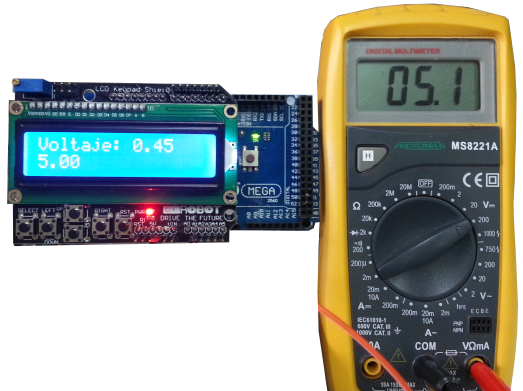
\includegraphics[scale=0.7]{images/arduino5.png}\caption{Ejemplo lectura Arduino}
			\end{figure}

			\begin{figure}[H]
			\centering
				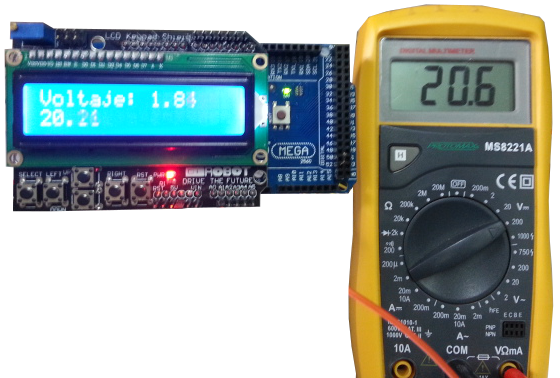
\includegraphics[scale=0.7]{images/arduino6.png}\caption{Ejemplo lectura Arduino}
			\end{figure}

		\subsection{Otras Opciones}

			Habiendo desarrollado una posible escalabilidad, se plantean tanto otras alternativas, como mejoras a la escalabilidad propuesta.

			\begin{itemize}
				\item \textbf{Fuente Variable:} Como plantea el proyecto de CEKIT, podemos construir una fuente variable utilizando el vúmetro como instrumento de medición de la tensión de salida.
				\item \textbf{Comandos locales / distancia:} Como se mencionó en la sección \ref{sec:func}, el conjunto Arduino-Raspberry con el shield LCD nos permitiría aplicar comandos no sólo por distancia sino también de manera local. De esta manera podriamos agregar un conjunto de funcionalidades / variaciones que se ejecuten por orden de estos comandos.
				\item \textbf{Comunicación Inalámbrica:} En el caso demostrado se utilizó comunicación cableada, lo cuál de necesitar cubrir grandes distancias puede ser ineficiente (o costoso) por lo cuál es preciso una comuniación inalámbrica. La Raspberry al tener un Linux embebido puede utilizar cualquier placa WiFi convencional. Para el Arduino es posible utilizar transmisores RF de bajo costo \footnote{Artículo en Mercado Libre \url{http://bit.ly/link_labo_rf}}.
			\end{itemize}


	\newpage\null\thispagestyle{empty}\newpage
	\section{Conclusiones}

	Se logró implementar el trabajo práctico deseado dentro de un tiempo prudente y se fue capaz de plantear y ejecutar una posibilidad de expansión del proyecto.

	Se elaboraron hipótesis y se corroboraron o corrigieron efectuando mediciones y aplicando los conceptos aprendidos durante la cursada y los trabajos prácticos previos. Además durante el transcurso de este proyecto, se aprendieron y aplicaron conceptos nuevos: diseño y confección de circuitos impresos, modelado de circuitos, servidores WEB, programación en Python y PHP, SSH, Arduino, Raspberry, entre otros. 

	Mediante el análisis de las variables (tensión de entrada y salida) comprendimos en que circunstancias un regulador de tensión opera adecuadamente. Asímismo analizamos el circuito y detectamos los componentes centrales que modificaban el comportamiento del vúmetro. Realizamos las mediciones pertinentes respecto a esos componentes, corroborando los datos teóricos obtenidos durante el diseño del circuito o en el caso de uno de los resistores, obtuvimos una discrepancia y la corregimos. Luego se planteó un método de medición de la escala empleando un divisor de tensión aparte de la posibilidad de utilizar la perilla reguladora de una fuente variable. 

	Conociendo que el circuito posee dos modos de trabajo, DOT y BAR, surgió la idea de analizar el consumo del circuito ya que la cantidad de LEDs a encender era muy diferente en uno u otro caso dependiendo la tensión mensurada. Se comentaron algunas hipótesis preliminares, luego de efectuadas las mediciones y analizando las gráficas obtenidas se concluyó que las hipótesis eran correctas; corroborando un incremento exponencial del consumo en modo BAR y lineal en modo DOT.

	Habiendo concluido el análisis técnico del circuito, se comentó cuales eran las ventajas y desventajas de utilizar un vúmetro cómo voltímetro, luego planteando una serie de mejoras y/o alternativas que resuelvan dichas desventajas. Uno de los casos que desarrollamos, fue la idea de pensar en las dificultades de aplicar una medición en un entorno industrial de gran escala y empleamos un Arduino y Raspberry como prototipo de sensor a distancia.

	Utilizando el Arduino (que posee un AVR Atmega 2560) fuimos capaces de tomar una lectura de tensión y mostrarla en una pantalla LED. Asímismo programamos una comunicación entre el Arduino y la Raspberry, permitiendonos sobre este último establecer una serie de funcionalidades como registro de lecturas para posterior análisis y consulta de lecturas vía web.

	Luego utilizando los mismo conceptos aplicados al vúmetro, analizamos la exactitud del mismo; corroborando las hipótesis mediante las cuales justificamos la realización de esta extensión.

	Tanto para el vúmetro como para la extensión se planteó una serie de especificaciones consideradas claves de los mismos y luego se fue capaz mediante las mediciones efectuadas corroborar las mismas, todas las especificaciones fueron satisfechas.

	\newpage\null\thispagestyle{empty}\newpage
	\section{Referencias}
		\label{sec:referencias}
		\begin{itemize}
		\item \textbf{Repositorio General} \url{https://github.com/aleperno/labotpfinal}
		\item \textbf{Especificaciones multímetro digital MS8221A} \url{https://github.com/aleperno/labotpfinal/raw/master/MS8221%20series.pdf}
		\item \textbf{Especificaciones multímetro digital Sonel CMM-40} \url{http://www.sonel.pl/sites/default/files/en/datasheet/datasheet_CMM-40_en_v1.pdf}
		\item \textbf{Hoja de datos LM3914} \url{https://github.com/aleperno/labotpfinal/raw/master/lm3914.pdf}
		\item \textbf{Hoja de datos LM7812} \url{https://github.com/aleperno/labotpfinal/raw/master/lm7805c.pdf}
		\item \textbf{Hoja de cálculos con Mediciones, Cálculos y Gráficos} \url{https://github.com/aleperno/labotpfinal/raw/master/tabla.ods}
		\item \textbf{Especificaciones Raspberry Pi B+} \url{https://www.adafruit.com/datasheets/pi-specs.pdf}
		\item \textbf{Especificaciones Arduino Mega 2560} \url{http://arduino.cc/en/Main/arduinoBoardMega2560}
		\item \textbf{Especifiaciones LCD Shield} \url{http://www.dfrobot.com/wiki/index.php?title=Arduino_LCD_KeyPad_Shield_(SKU:_DFR0009)}
		\item \textbf{Gráficos Arduino y Protobard} \url{http://fritzing.org/home/}
		\item \textbf{Código Fuente Arduino} \url{https://github.com/aleperno/labotpfinal/blob/master/src/labo.ino}
		\item \textbf{Código Fuente Raspberry} \url{https://github.com/aleperno/labotpfinal/blob/master/src/labo.py}
		\item \textbf{Código Fuente PHP} \url{https://github.com/aleperno/labotpfinal/blob/master/src/index.php}
		\item \textbf{Código Fuente Grafico Python} \url{https://github.com/aleperno/labotpfinal/blob/master/src/graf.py}
		\end{itemize}

	\newpage\null\thispagestyle{empty}\newpage
	\section{Anexo}\label{sec:anexo}
		\subsection{Mulímetro Digital MS8221A}
		\begin{figure}[H]
			\centering
				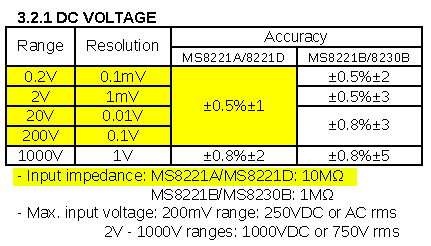
\includegraphics[scale=1.5]{attachments/dvm_specs.pdf}\caption{Especificaciones DVM}
			\end{figure}

		\begin{figure}[H]
			\centering
				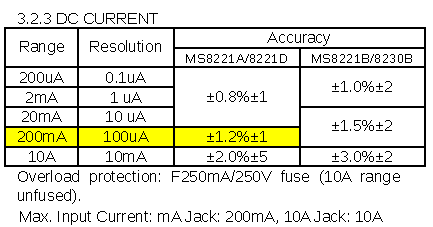
\includegraphics[scale=1.5]{attachments/dvm_specs1.pdf}\caption{Especificaciones DVM}
			\end{figure}

		\subsection{LM3914}
		\begin{figure}[H]
			\centering
				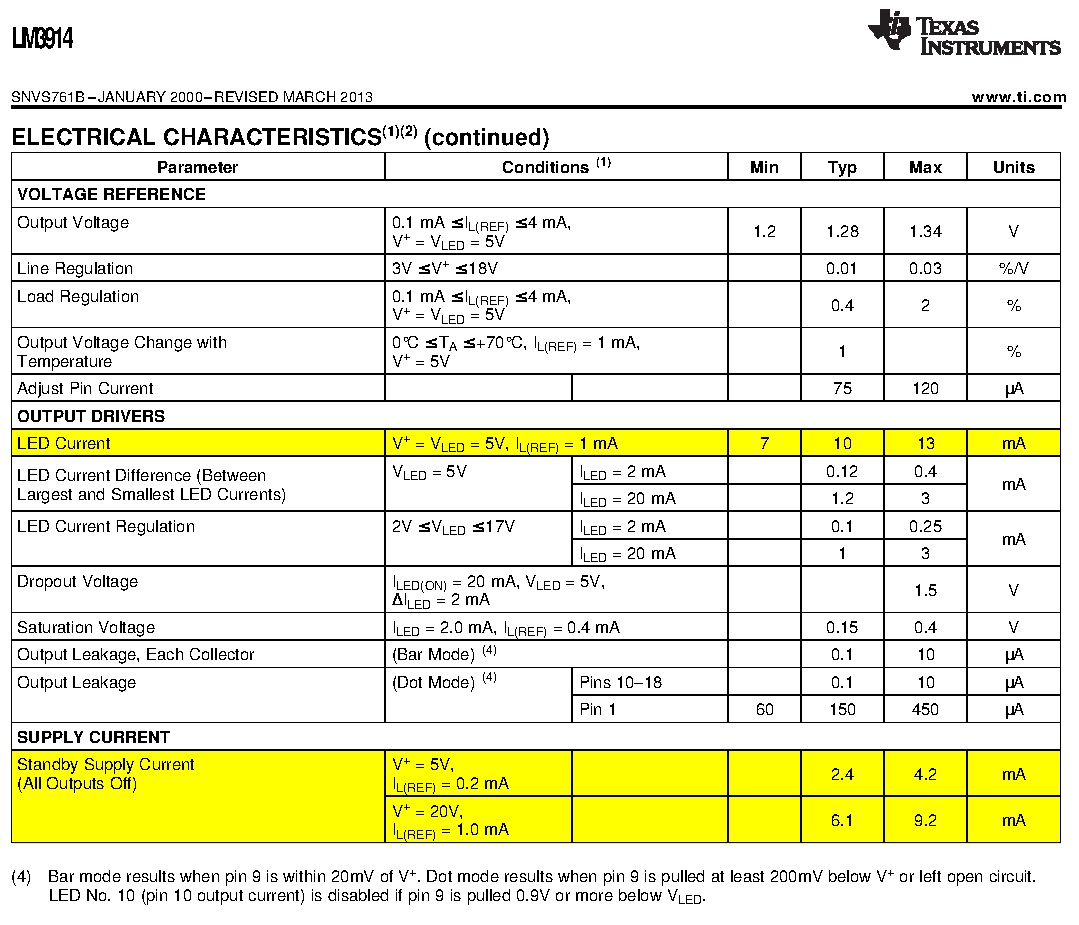
\includegraphics[scale=1]{attachments/lm3914_specs.pdf}\caption{Especificaciones LM3914}
			\end{figure}

		\subsection{LM7812}
		\begin{figure}[H]
			\centering
				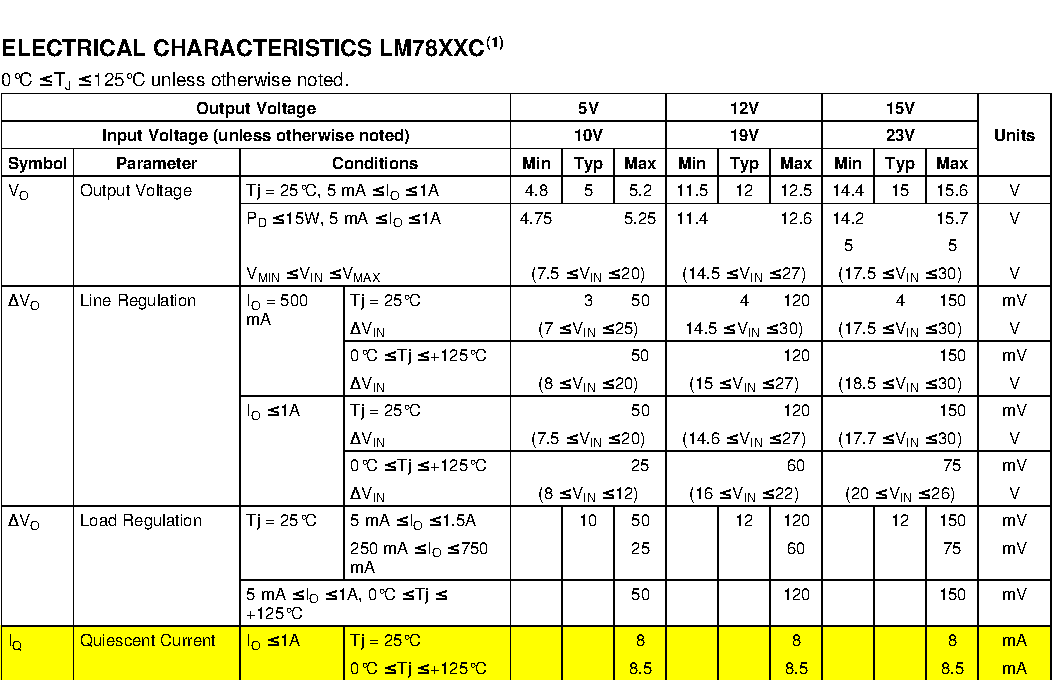
\includegraphics[scale=0.9]{attachments/lm7805c_specs.pdf}\caption{Especificaciones DVM}
			\end{figure}

		\begin{figure}[H]
			\centering
				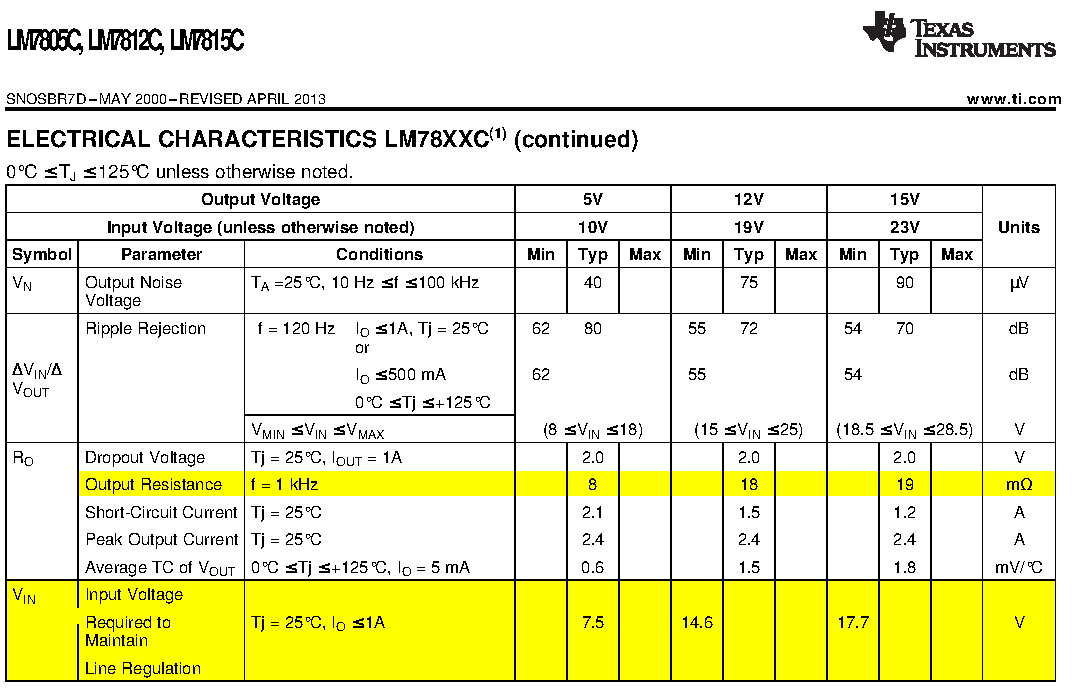
\includegraphics[scale=0.9]{attachments/lm7805c_specs2.pdf}\caption{Especificaciones DVM}
			\end{figure}

\end{document}
